\section{Diseño e implementación de las bases de datos}
\label{sec:diseñoImplementacionBasesDeDatos}

En base a la información a modelar se ha decidido utilizar tres bases de datos, una por cada archivo del simulador ROBIN, es decir, una para los datos de los archivos que definen la oferta del día que se va a simular, otra para los datos de la configuración de la demanda esperada para ese día y, por último, una que recoge los resultados de las simulaciones realizadas.

Dado que estas tres bases de datos comparten una estructura similar, se va a proceder a detallar el esquema común utilizando nombre de claves genéricos que indican el nivel dónde se encuentra la clave (raíz 1, raíz 2, raíz 2.2, etc.) (Figura~\ref{fig:DiagramaEstructuraBaseDeDatos}). Como se puede observar, los datos que referencian la clave raíz 1 se almacenan únicamente en una tabla, mientras que los datos de la clave raíz 2, se almacenan en dos tablas, donde una almacenan los datos que referencian las claves 2.1, 2.2, 2.3, 2.4, 2.5 y 2.6, mientras que en la tabla de datos auxiliar se almacenan los datos que asociados a la clave 2.7.

\begin{figure}[H]
\centering
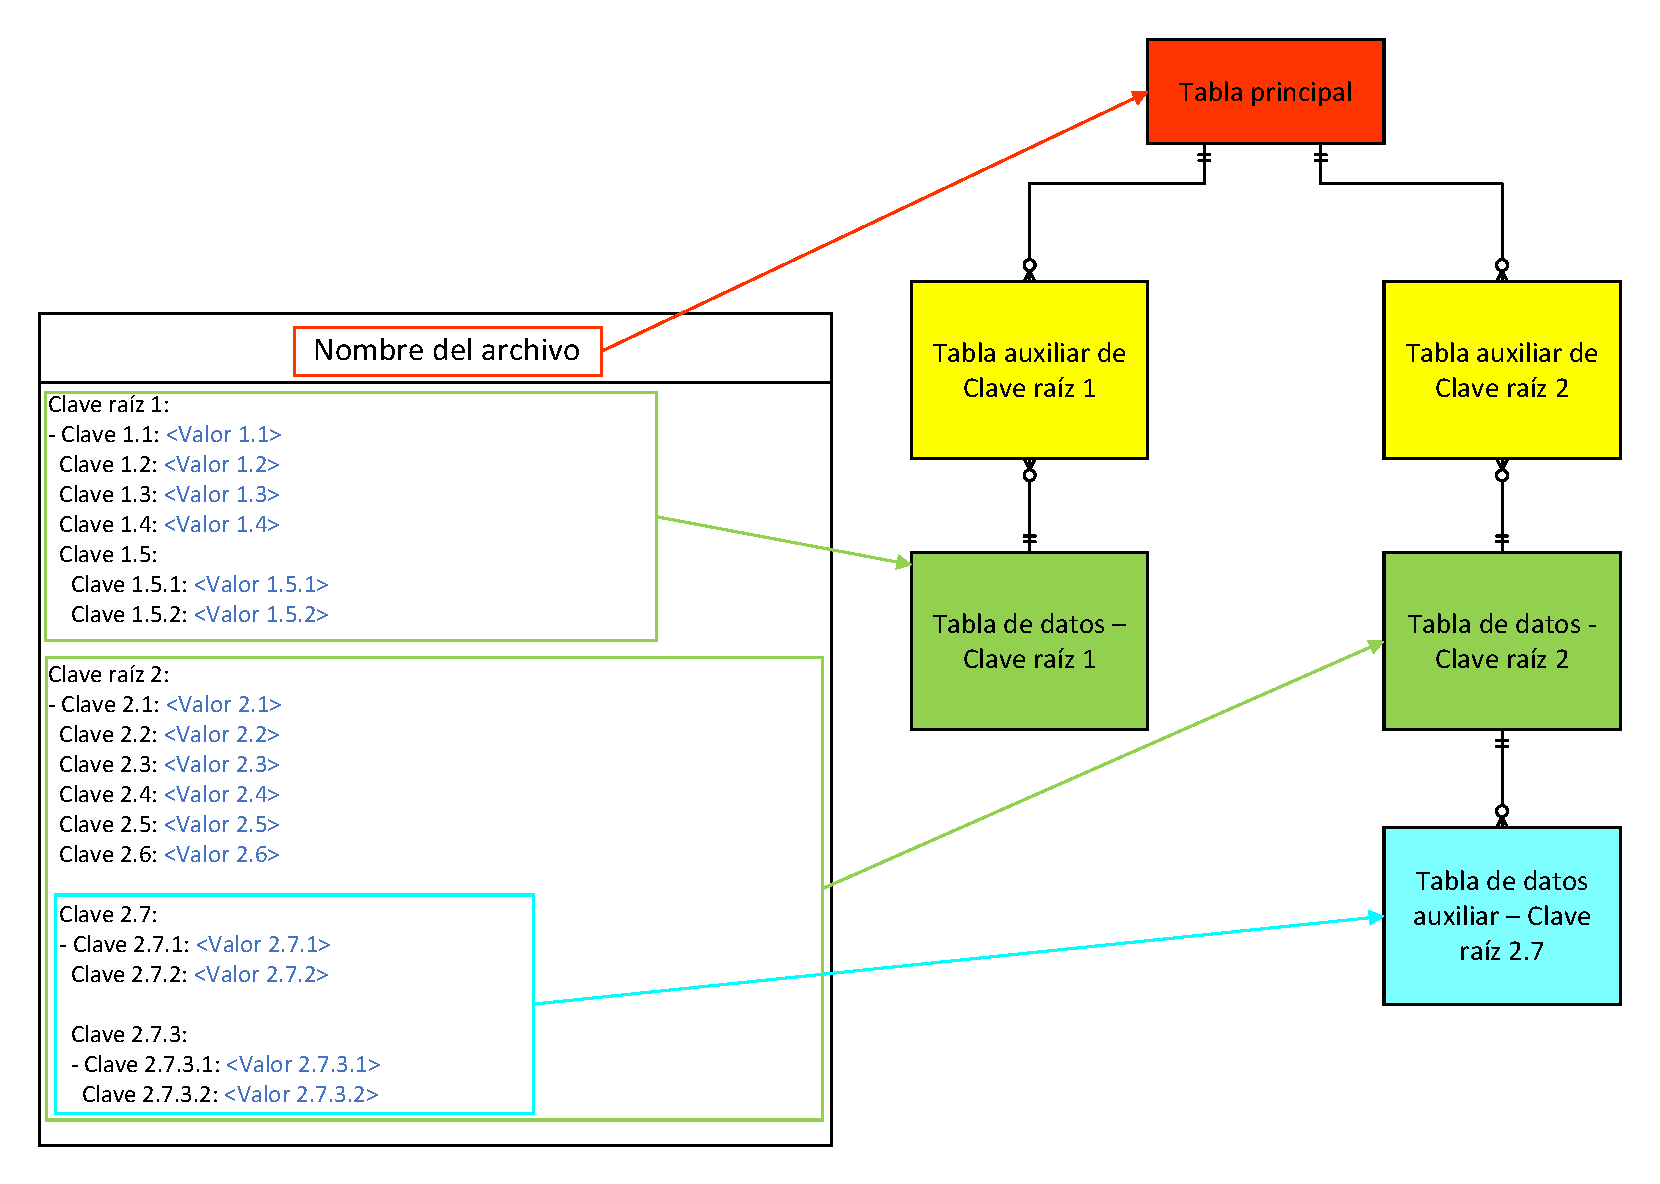
\includegraphics[width=1\textwidth]{fig/Diagramas/Estructura bases de datos.pdf}
\caption{Diagrama de la estructura de las bases de datos. En naranja aparece la tabla principal, en amarillo las tablas auxiliares, en verde las tablas de datos y en azul las tablas de datos auxiliares.}
\label{fig:DiagramaEstructuraBaseDeDatos}
\end{figure}

La tabla principal (en naranja en la figura) almacena el nombre del archivo y las observaciones pertinentes. El objetivo de estas tablas consiste en tener un punto de partida para la reconstrucción de los archivos empleando los datos almacenados en la base de datos. Esto se lleva a cabo mediante el uso de los identificadores que se asignan a cada uno de los archivos y unas tablas auxiliares que conectan la información contenida en las demás tablas de la base de datos con la tabla principal. La tabla principal tiene las siguientes columnas: %y que contiene las siguientes tres columnas: 
\begin{enumerate}
    \item La primera es para el identificador que se le asigna a cada fila. Este proceso se realiza de forma automática.
    \item Otra que almacena el nombre del archivo sin la extensión del mismo.
    \item Finalmente, una columna para guardar las observaciones realizadas para cada archivo, en caso de que existieran.
\end{enumerate}

De esta tabla dependen varias tablas auxiliares, cuyo cometido, como ya se ha mencionado anteriormente, es el de relacionar los archivos con la información perteneciente a dichos archivos, asociando el identificador de la entrada que pertenece a cada archivo con los identificadores de la información perteneciente a dicho archivo. 

Por último, se cuenta con las tablas destinadas a albergar los datos. Estas tablas contienen una estructura similar a la que se emplea en los archivos. En el caso de los archivos \acrshort{Yaml}, existen tablas que no dependan de otras, que vendrán definidas por las claves raíz dentro de los archivos.

%Además, existirán otras tablas de datos que dependan de estas primeras \textbf{TEMA: DE CUALES? ES UN LÍO, EXPLICA BIEN CON EL ESQUEMA} en las que se almacenan los datos de claves que dentro del archivo tengan anidadas más claves. Esta estructura ayuda a que las sentencias \acrshort{SQL} funcionen de una mejor forma, posibilitando sentencias \acrshort{SQL} más sencillas.

Además, existen unas tablas de datos auxiliares, que dependen de las tablas de datos, en las que se almacenan datos de estructuras más complejas que puedan aparecer en los archivos \acrshort{Yaml}, como un diccionario que tenga otro diccionario anidado o una lista de diccionarios. Esta estructura ayuda a que las sentencias \acrshort{SQL} sean más sencillas.

En resumen, se ha diseñado como un acceso tipo jerárquico a tres niveles, se puede decir, como ``en forma de árbol'', contando con una tabla de datos auxiliar final, en caso de ser necesario.

%se compliquen más de lo necesario, porque estos datos anidados se podrían almacenar como un texto en formato \acrshort{JSON}, pero para extraer los valores para realizar una consulta a la base de datos, la sentencia \acrshort{SQL} necesaria sería muy complicada de diseñar. 

A continuación, se mostrará un ejemplo de algunas tablas de la estructura de la Figura~\ref{fig:DiagramaEstructuraBaseDeDatos}.

En la Figura~\ref{fig:ColumnasTablaPrincipal} se pueden ver las columnas de todas las tablas principales. Esta tabla contiene las columnas \texttt{ID}, en la que aparece un identificador único, generado automáticamente para cada una de las filas, que actúa como clave primaria, \texttt{NAME}, que almacena el nombre del archivo y \texttt{OBSERVATIONS}, en el que se guardan las observaciones para el archivo.

\begin{figure}[H]
\centering
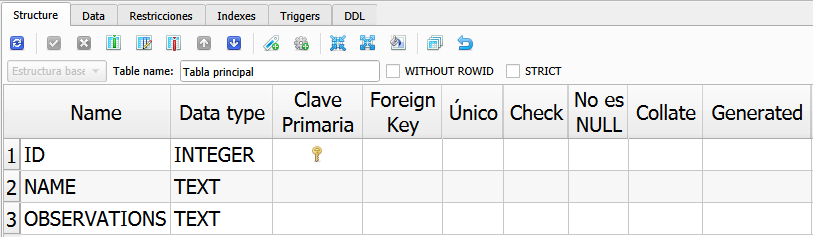
\includegraphics[width=1\textwidth]{fig/Base de datos estructura/Columnas tabla principal.png}
\caption{Columnas de la tabla principal.}
\label{fig:ColumnasTablaPrincipal}
\end{figure}

La Figura~\ref{fig:ColumnasTablaDatosClaveRaiz1} muestra las columnas de la tabla destinada a almacenar los datos a los que se hace referencia en la clave raíz 1 que aparecen en la Figura~\ref{fig:DiagramaEstructuraBaseDeDatos}. Esta cuenta con una columna \texttt{ID} que es una clave primaria con un valor numérico generado de manera autoincremental y las demás columnas contienen los datos asociados a cada una de las claves dentro de la clave raíz 1. Para el caso de la clave 1.5, que hace referencia a un diccionario, se almacena en la columna con el nombre de \texttt{CLAVE\_1.5} y tipo de datos diccionario (\textit{JSON}). 

\begin{figure}[H]
\centering
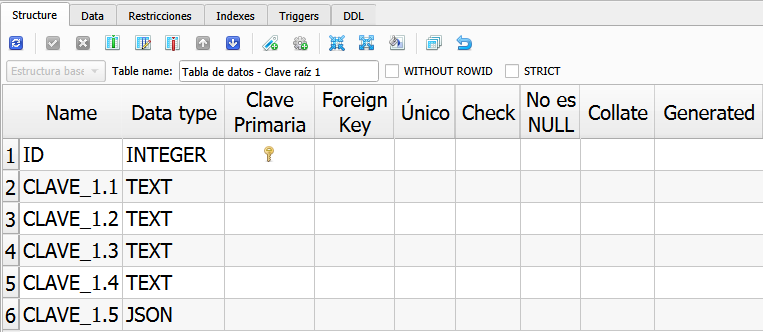
\includegraphics[width=.9\textwidth]{fig/Base de datos estructura/Columnas tabla de datos clave raiz 1.png}
\caption{Columnas de la tabla de datos de la clave raíz 1.}
\label{fig:ColumnasTablaDatosClaveRaiz1}
\end{figure}

La Figura~\ref{fig:ColumnasTablaDatosClaveRaiz2} muestra los datos asociados a la clave raíz 2 que aparecen en la Figura~\ref{fig:DiagramaEstructuraBaseDeDatos}. Cuenta con una columna \texttt{ID} que almacena el identificador autoincremental asignado a cada fila de forma automática, mientras que las demás columnas contienen los datos asociados a las claves bajo la clave raíz 2, a excepción de los datos referenciados por la clave 2.7 que se almacenan en una tabla distinta, pero relacionada con esta mediante la columna \texttt{ID}.

\begin{figure}[H]
\centering
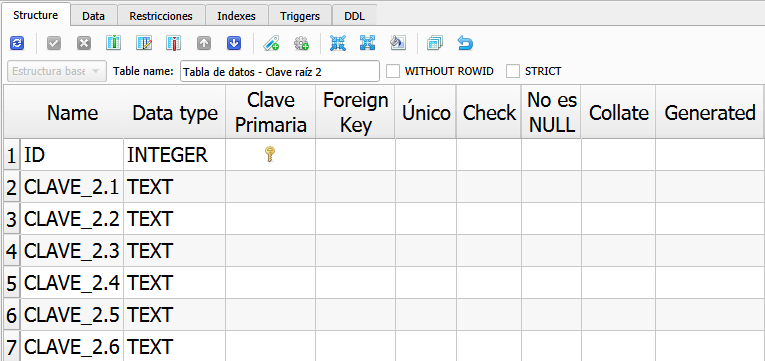
\includegraphics[width=.9\textwidth]{fig/Base de datos estructura/Columnas tabla de datos clave raiz 2.png}
\caption{Columnas de la tabla de datos de la clave raíz 2.}
\label{fig:ColumnasTablaDatosClaveRaiz2}
\end{figure}

En la Figura~\ref{fig:ColumnasTablaDatosAuxiliarClaveRaiz2} se muestran las columnas de la tabla auxiliar de datos de la clave raíz 2, destinada a contener los datos asociados a la clave 2.7. 
%Esto se ha hecho así, porque la estructura asociada a la clave 2.7 es algo más compleja que la que aparece bajo la clave 1.5 asociada a la clave raíz 1. Aunque se puede guardar en formato \acrshort{JSON} en una única columna, esto a la hora de crear las sentencias \acrshort{SQL} para extraer datos de esta columna ficticia, resultaría complicado y por eso se ha optado por separar la información en dos tablas.
Esta tabla tiene definida una relación con la tabla de datos de la clave raíz 2 (Figura~\ref{fig:ColumnasTablaDatosClaveRaiz2}) mediante la clave foránea que se almacena en la columna \texttt{TABLA\_CLAVE\_RAIZ\_2\_ID} y que contiene el identificador de la tabla de datos de la clave raíz 2 con la que los datos de la fila de la tabla de datos auxiliar guardan relación.

\begin{figure}[H]
\centering
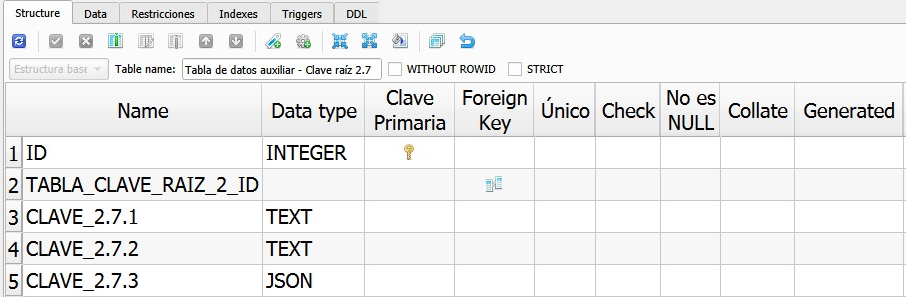
\includegraphics[width=.9\textwidth]{fig/Base de datos estructura/Columnas tabla de datos auxiliar clave raiz 2.png}
\caption{Columnas de la tabla de datos auxiliar de la clave raíz 2 con los datos asociados a la clave 2.7.}
\label{fig:ColumnasTablaDatosAuxiliarClaveRaiz2}
\end{figure}

En las Figuras \ref{fig:ColumnasTablaAuxiliarClaveRaiz1} y \ref{fig:ColumnasTablaAuxiliarClaveRaiz2} se pueden ver las tablas auxiliares destinadas a relacionar los datos de las tablas de datos con la tabla principal. Para el caso de la tabla auxiliar de la clave raíz 1 (Figura~\ref{fig:ColumnasTablaAuxiliarClaveRaiz1}), relaciona la tabla principal con la tabla de datos de la clave raíz 1, mediante una relación establecida utilizando los identificadores de ambas tablas. Esta relación se materializa a través de las claves foráneas almacenadas en las columnas \texttt{TABLA\_PRINCIPAL\_ID}, para el identificador de la tabla principal y \texttt{TABLA\_CLAVE\_RAIZ\_1\_ID}, para el identificador de la tabla de datos de la clave raíz 1.

\begin{figure}[H]
\centering
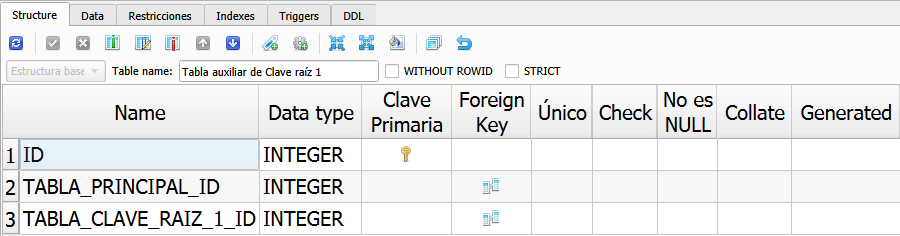
\includegraphics[width=.9\textwidth]{fig/Base de datos estructura/Columnas tabla auxiliar de clave raiz 1.png}
\caption{Columnas de la tabla auxiliar de la clave raíz 1.}
\label{fig:ColumnasTablaAuxiliarClaveRaiz1}
\end{figure}

La tabla auxiliar de la clave raíz 2 (Figura~\ref{fig:ColumnasTablaAuxiliarClaveRaiz2}) funciona de manera similar a la anterior, pero relaciona los datos de la tabla principal con los datos de la tabla de datos de la clave raíz 2, y a su vez, con la tabla auxiliar de datos de la clave raíz 2 debido a que las dos tablas de datos están relacionadas entre sí. La relación entre la tabla principal y la tabla de datos de la clave raíz 2 se lleva a cabo mediante claves foráneas almacenadas en las columnas \texttt{TABLA\_PRINCIPAL\_ID} y \texttt{TABLA\_CLAVE\_RAIZ\_1\_ID}, respectivamente.

\begin{figure}[H]
\centering
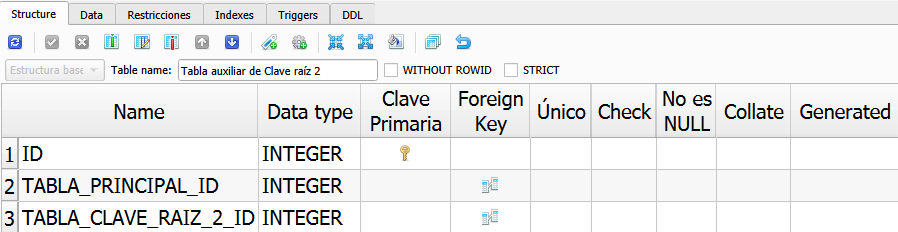
\includegraphics[width=.9\textwidth]{fig/Base de datos estructura/Columnas tabla auxiliar de clave raiz 2.png}
\caption{Columnas de la tabla auxiliar de la clave raíz 2.}
\label{fig:ColumnasTablaAuxiliarClaveRaiz2}
\end{figure}

\begin{comment}
Por ejemplo \textbf{TEMA: UN EJEMPLO DE QUÉ? DE LAS CONSULTAS QUE ES LO ÚLTIMO QUE HAS DICHO?}, la clave almacena un único diccionario y este es relativamente sencillo, como en el caso de las coordenadas, bajo la clave \texttt{coordinates}, de las estaciones en la \textbf{clave raíz} \texttt{stations} (Listado~\ref{src:estructuraYamlOfertaStations}) del archivo de configuración de la oferta, esta sí que se almacena como un texto en formato \acrshort{JSON} (Véase la figura~\ref{fig:dbSupplySTATIONSWithData}).

\begin{lstlisting}[language=YAML,
                   frame=none,
                   numbers=none,
                   basicstyle=\ttfamily\normalsize,
                   caption={Estructura de la \textbf{clave raíz} \texttt{stations}},
                   label=src:estructuraYamlOfertaStations,
                   inputencoding=utf8]                   
#Lista con los datos de las estaciones
stations:
- id: <Identificador de la estación>
  name: <Nombre de la estación>
  city: <Ciudad en la que se encuentra la estación>
  short_name: <Nombre corto de la estación>
  coordinates:
    latitude: <Latitud a la que se encuentra la estación>
    longitude: <Longitud a la que se encuentra la estación>
\end{lstlisting}

\begin{figure}[H]
\centering
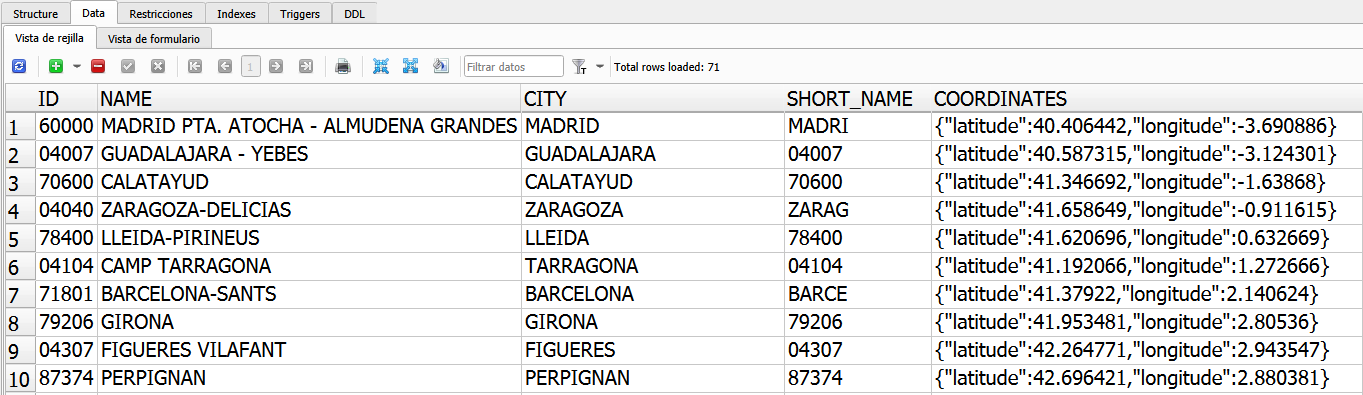
\includegraphics[width=1\textwidth]{fig/Datos reales de las tablas/STATIONS_DATA.png}
\caption{Tabla \texttt{STATIONS} con datos reales.}
\label{fig:dbSupplySTATIONSWithData}
\end{figure}

Por el contrario, la clave \texttt{origin\_destination\_tuples} dentro de la \textbf{clave raíz} \texttt{service} (Listado~\ref{src:estructuraYamlOfertaService}) tiene un diccionario más complejo que el antes mencionado, por lo que se ha optado por guardar la información de esta clave en otra tabla, bajo el nombre de \texttt{ORIGIN\_DESTINATION\_TUPLES}. 

\begin{lstlisting}[language=YAML,
                   frame=none,
                   numbers=none,
                   basicstyle=\ttfamily\normalsize,
                   caption={Estructura de la \textbf{clave raíz} \texttt{service}},
                   label=src:estructuraYamlOfertaService,
                   inputencoding=utf8]                   
#Lista con la información de los servicios
service:
- id: <Identificador del servicio>
  date: <Fecha en la que se da el servicio>
  line: <Linea a la que pertenece el servicio>
  train_service_provider: <Proveedor encargado del servicio>
  time_slot: <Franja horaria de inicio del servicio>
  rolling_stock: <Tren que va a cumplir el servicio>
  
  #Lista con la información de los trayectos entre estaciones del servicio
  origin_destination_tuples:
  - origin: <Estación de origen>
    destination: <Estación de destino>
    
    #Lista con el precio de cada asiento
    seats:
    - seat: <Identificador del asiento>
      price: <Precio del asiento para el trayecto>
  capacity_constraints: <Restricción de capacidad, null en caso de no existir>
\end{lstlisting}

\begin{figure}[H]
\centering
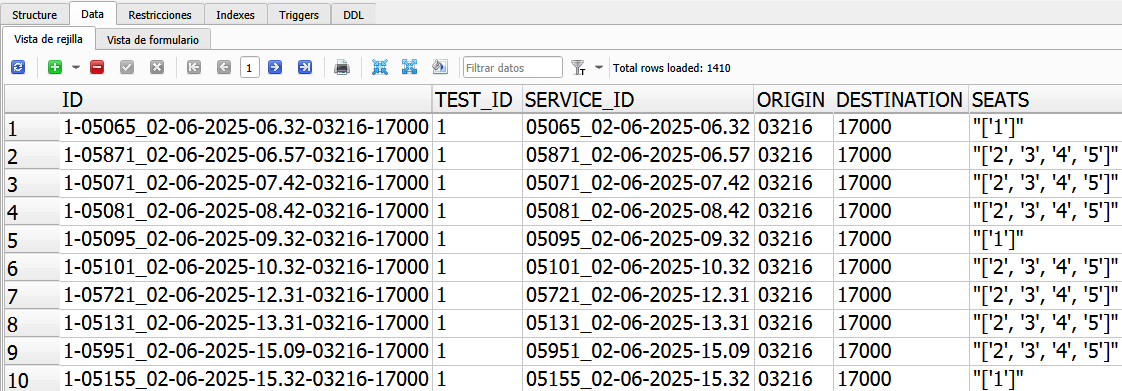
\includegraphics[width=1\textwidth]{fig/Datos reales de las tablas/ORIGIN_DESTINATION_TUPLES_DATA.png}
\caption{Tabla \texttt{ORIGIN\_DESTINATION\_TUPLES} con datos reales.}
\label{fig:dbSupplySTATIONSWithData}
\end{figure}

En el caso de la clave \texttt{origin\_destination\_tuples}, el precio de los asientos se ha separado de la tabla \texttt{ORIGIN\_DESTINATION\_TUPLES} y los datos del precio se han almacenado en otra tabla llamada \texttt{SEATS\_PRICE} (Figura~\ref{fig:dbSupplySEATS_PRICEWithData}). Esto se ha hecho así para evitar que en la tabla \texttt{ORIGIN\_DESTINATION\_TUPLES} aparecieran estructuras de datos complejas, debido a que cada precio está asociado a un asiento concreto, que puede aparecer o no, dentro de la clave \texttt{seats}, lo que complicaría mucho la consulta de la información del precio de los asientos mediante sentencias \acrshort{SQL}, ya que no hay una clave fija de la que extraer la información, como en el caso de las coordenadas de las estaciones dentro de la \textbf{clave raíz} \texttt{stations}, sino que las claves que se usan para definir los precios, aunque se sabe que tienen que ser los identificadores de los tipos de asiento, nada garantiza que estén todos los identificadores de los asientos, por lo que es imposible conocer con certeza qué asientos tienen un precio asignado para los trayectos definidos en la clave \texttt{origin\_destination\_tuples} de una manera sencilla.

\begin{figure}[H]
\centering
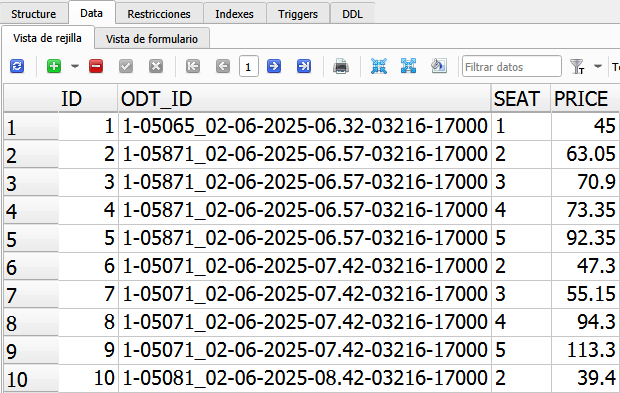
\includegraphics[width=0.7\textwidth]{fig/Datos reales de las tablas/SEATS_PRICE_DATA.png}
\caption{Tabla \texttt{SEATS\_PRICE} con datos reales.}
\label{fig:dbSupplySEATS_PRICEWithData}
\end{figure}
\end{comment}

Todas las figuras de las tablas pertenecientes a las bases de datos han sido capturadas del programa SQLiteStudio~\cite{SQLiteStudio}. Este programa se ha empleado en el diseño, visualización y realización de las pruebas pertinentes en las diferentes bases de datos empleadas en este \acrshort{TFG}.

Finalmente, indicar que en el caso de los archivos de resultados, la tabla de datos tendrá las mismas columnas que los archivos \acrshort{CSV} que se generan al acabar la simulación con \acrshort{ROBIN}.

\subsection{Base de datos para los archivos de entrada de datos de la oferta}
\label{subsec:dBSupply}

La base de datos que contiene los datos de la configuración de la oferta consta de 21 tablas, cuya organización aparece en el \acrfull{EDR} mostrado en la Figura~\ref{fig:edrOfertaSimplificado}). Una versión más extendida de dicho \acrshort{EDR}, que contiene también los nombres de las columnas de cada una de las tablas, se encuentra  en el Anexo~\ref{fig:edrOferta}. Esta base de datos almacena los datos relacionados con la oferta de servicios ferroviarios correspondientes a un rango de tiempo determinado, que puede abarcar desde un día hasta varios. Estos datos se emplean en el simulador \acrshort{ROBIN} para definir la oferta disponible en base al archivo de configuración de la oferta.

\begin{figure}[H]
\centering
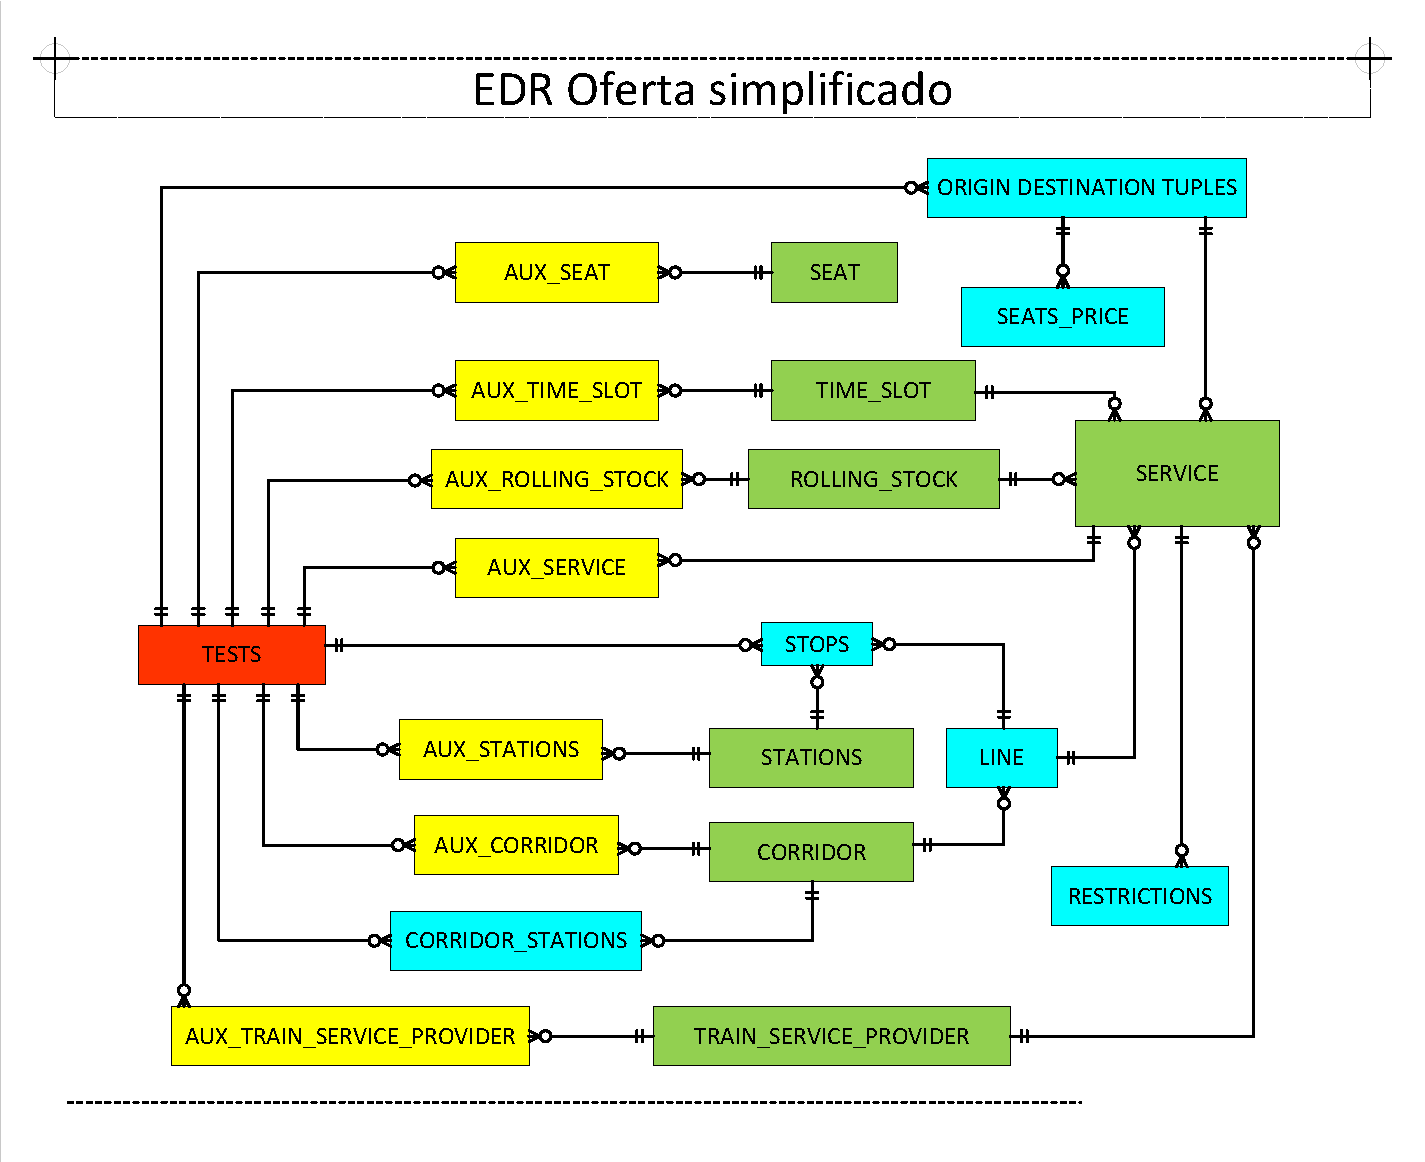
\includegraphics[width=.9\textwidth]{fig/Bases de datos/EDR oferta simplificado.pdf}
\caption{Esquema de la base de datos para archivos de entrada de datos de la oferta. En naranja aparece la tabla principal, en amarillo las tablas auxiliares, en verde las tablas de datos y en azul las tablas de datos auxiliares.}
\label{fig:edrOfertaSimplificado}
\end{figure}

La tabla principal de la base de datos aparece representada con el color naranja y tiene la finalidad de almacenar el nombre de los archivos \acrshort{Yaml} de entrada de datos de la oferta importados a la base de datos y las observaciones que el usuario estime pertinentes.

Las tablas auxiliares aparecen en color amarillo. Estas tablas relacionan los datos almacenados en las tablas de la base de datos con el archivo de oferta al que pertenecen mediante los identificadores que poseen. Esto evita elementos repetidos en las tablas de datos, optimizando el espacio que ocupan los datos dentro de la base de datos. De esta manera, si una clave raíz tiene asociados los mismos datos en dos archivos diferentes, estos datos solo aparecen reflejados una vez en las tablas de datos y, empleando la tabla auxiliar correspondiente a esta clave raíz, se asocia el dato común a ambos archivos. Por ejemplo, si en dos archivos \acrshort{Yaml} diferentes, bajo la clave raíz que referencia a las estaciones aparece la estación de Madrid Puerta de Atocha - Almudena Grandes, en la tabla de datos dedicada a almacenar los datos de las estaciones aparece una única vez, mientras que en la tabla auxiliar aparece el identificador perteneciente a la estación mencionada dos veces, debido a que se encuentra asociado a dos archivos diferentes. Además, estas tablas auxiliares son la base desde la que se reconstruyen los archivos a la hora de exportarlos, ya que relacionan toda la información de las tablas de datos con el archivo \acrshort{Yaml} del que provienen.

Las tablas de datos, de color verde, tienen la función de albergar los datos asociados a las diferentes claves raíz del archivo \acrshort{Yaml} de entrada de datos de la oferta, por ejemplo, los datos de las estaciones, las líneas de tren o los servicios ferroviarios, entre otros. Si bajo alguna de estas claves raíz se encuentra referenciada una estructura más compleja (por ejemplo, la clave \texttt{origin\_destination\_tuples} asociada a la clave raíz \texttt{service}) se almacena en las tablas de datos auxiliares, que en el diagrama de la Figura~\ref{fig:edrOfertaSimplificado} aparecen de color azul claro. Esto facilita la creación de sentencias \acrshort{SQL}, dado que no hay que trabajar con texto en formato \acrshort{JSON}. Otras estructuras de datos más simples como listas o diccionarios se han introducido como texto en formato \acrshort{JSON} en las tablas de datos, como por ejemplo, en la tabla de datos de las estaciones, en la que aparecen las coordenadas de las estaciones como un diccionario con las claves \texttt{latitude} y \texttt{longitude}. En este caso, es relativamente sencillo obtener los datos de este diccionario ya que las claves son conocidas y bajo estas claves no se referencia ninguna otra estructura de datos, sino valores numéricos. Un ejemplo de cómo extraer los datos de estas columnas aparecerá más adelante cuando se explique la estructura de la tabla de datos de las estaciones.

A continuación se muestra cada una de las tablas que componen esta base de datos.

\subsubsection{Tabla principal}
La tabla principal de la base de datos es la tabla \texttt{TESTS} (Figura~\ref{fig:dbSupplyTESTS}). En dicha tabla, se almacenan el nombre del archivo introducido en la base de datos y las posibles observaciones que el usuario estime pertinentes. Además, a cada archivo introducido se le añade un identificador único, que es la clave primaria de la tabla y que se emplea como clave foránea o externa en otras tablas para establecer las relaciones con la tabla principal.

\begin{figure}[H]
\centering
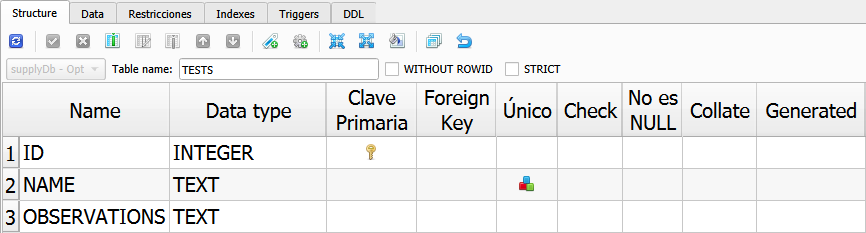
\includegraphics[width=.9\textwidth]{fig/Tablas base de datos/Oferta/TESTS.png}
\caption{Tabla principal de la base de datos para archivos de oferta.}
\label{fig:dbSupplyTESTS}
\end{figure}

En la Figura~\ref{fig:dbSupplyTESTSWithData} se pueden observar cómo están almacenados los datos en la tabla de la Figura~\ref{fig:dbSupplyTESTS}. La información que se puede ver en la Figura~\ref{fig:dbSupplyTESTSWithData} se corresponde con la de los archivos \acrshort{Yaml} de configuración de la oferta, en este caso, el nombre del archivo empleado. 

\begin{figure}[H]
\centering
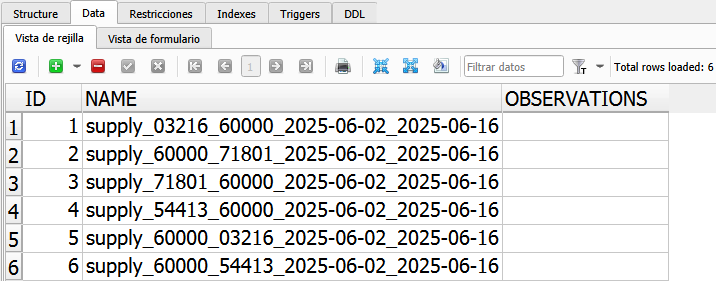
\includegraphics[width=.9\textwidth]{fig/Datos reales de las tablas/TESTS_DATA.png}
\caption{Ejemplo con datos reales de la tabla~\ref{fig:dbSupplyTESTS}.}
\label{fig:dbSupplyTESTSWithData}
\end{figure}

\subsubsection{Tablas de datos}

Esta base de datos incluye varias tablas destinadas a almacenar la información proveniente de los archivos de configuración de la oferta. Dichos archivos contienen información relacionada con, por ejemplo, las estaciones que se encuentran en el corredor y las líneas que aparecen en los servicios ofertados por las compañías proveedoras de servicios ferroviarios.

La tabla \texttt{STATIONS} (Figura~\ref{fig:dbSupplySTATIONS}) contiene los datos relacionados con las estaciones que aparecen en las diferentes líneas de los servicios ferroviarios. 

Los campos de esta tabla son: 
\begin{itemize}
    \item \texttt{ID}: Identificador único de la estación.
    \item \texttt{NAME}: Nombre de la estación.
    \item \texttt{CITY}: Ciudad donde está ubicada la estación.
    \item \texttt{SHORT\_NAME}: Nombre corto de la estación.
    \item \texttt{COORDINATES}: Coordenadas geográficas de la estación.
\end{itemize}

La mayoría de las columnas de la tabla contienen datos en formato de texto plano, excepto en el caso de la columna \texttt{COORDINATES}, que utiliza un formato \acrfull{JSON} para almacenar la latitud y la longitud en un único campo.

\begin{figure}[H]
\centering
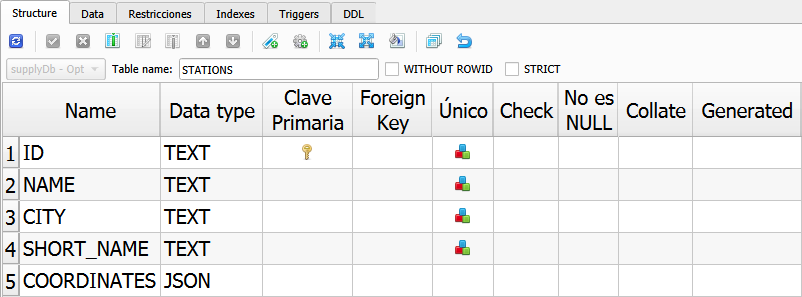
\includegraphics[width=.9\textwidth]{fig/Tablas base de datos/Oferta/STATIONS.png}
\caption{Tabla \texttt{STATIONS}}
\label{fig:dbSupplySTATIONS}
\end{figure}

A continuación, se muestra cómo extraer los datos de las coordenadas de las estaciones empleando una sentencia \acrshort{SQL}. El Listado~\ref{src:extraerInfoDeEStaciones} detalla cómo usar el comando \texttt{json\_extract} para obtener la latitud y la longitud de la columna \texttt{COORDINATES} de la tabla \texttt{STATIONS} que tiene asignado el tipo \acrshort{JSON} como tipo de datos. En este caso, esa columna almacena un diccionario con las claves \texttt{latitude} y \texttt{longitude} en las que se almacenan los valores de la latitud y longitud, respectivamente, a las que se encuentra la estación.

\lstinputlisting[language=SQL, frame=none, numbers=none, basicstyle=\ttfamily\normalsize, caption=Sentencia                         SQL para extraer los datos de las estaciones dentro de la tabla \texttt{STATIONS}, 
                 label=src:extraerInfoDeEStaciones, inputencoding=utf8]{auxFiles/Querys de ejemplos/Extraer info de estaciones.sql}

Como el listado de estaciones es extenso, se ha tomado una muestra con las 5 primeras filas del archivo \acrshort{CSV} generado a partir de la sentencia del Listado~\ref{src:extraerInfoDeEStaciones}. Esta muestra se encuentra en la tabla~\ref{tab:extraerInfoDeEStaciones}. El archivo \acrshort{CSV} que contiene todas las entradas generadas mediante la sentencia \acrshort{SQL} se puede encontrar en el siguiente \href{https://github.com/Sergioba99/TFG-Gestor_De_Bases_de_Datos/blob/master/Archivos%20Yaml%20y%20CSV/Exportados/Vistas%20exportadas/Extraer%20info%20de%20estaciones.csv}{enlace}\footnote{\url{https://github.com/Sergioba99/TFG-Gestor\_De\_Bases\_de\_Datos/blob/master/Archivos\%20Yaml\%20y\%20CSV/Exportados/Vistas\%20exportadas/Extraer\%20info\%20de\%20estaciones.csv}}.

\begin{table}[H]
\centering
\small
\setlength\tabcolsep{3pt}
\resizebox{\textwidth}{!}{
\begin{tabular}{l|l|c|c|c|c|c|}
  \cline{2-7}
   & \multicolumn{1}{c|}{\cellcolor[HTML]{C0C0C0}ID}
   & \multicolumn{1}{c|}{\cellcolor[HTML]{C0C0C0}NAME}
   & \multicolumn{1}{c|}{\cellcolor[HTML]{C0C0C0}CITY}
   & \multicolumn{1}{c|}{\cellcolor[HTML]{C0C0C0}SHORT\_NAME}
   & \multicolumn{1}{c|}{\cellcolor[HTML]{C0C0C0}LATITUD}
   & \multicolumn{1}{c|}{\cellcolor[HTML]{C0C0C0}LONGITUD} \\ \hline
  \multicolumn{1}{|l|}{1} & 60000 & MADRID PTA. ATOCHA – ALMUDENA GRANDES & MADRID    & MADRI & 40.406442 & –3.690886  \\ \hline
  \multicolumn{1}{|l|}{2} & 04007 & GUADALAJARA – YEBES                  & GUADALAJARA & 04007 & 40.587315 & –3.124301  \\ \hline
  \multicolumn{1}{|l|}{3} & 70600 & CALATAYUD                            & CALATAYUD   & 70600 & 41.346692 & –1.638680  \\ \hline
  \multicolumn{1}{|l|}{4} & 04040 & ZARAGOZA-DELICIAS                   & ZARAGOZA    & ZARAG & 41.658649 & –0.911615  \\ \hline
  \multicolumn{1}{|l|}{5} & 78400 & LLEIDA-PIRINEUS                      & LLEIDA      & 78400 & 41.620696 &  0.632669  \\ \hline
\end{tabular}}
\caption{Primeras cinco filas de la salida de la sentencia SQL del Listado~\ref{src:extraerInfoDeEStaciones}}
\label{tab:extraerInfoDeEStaciones}
\end{table}

Los datos de los diferentes proveedores de servicios ferroviarios que puedan existir se registran en la Tabla \texttt{TRAIN\_SERVICE\_PROVIDER} (Figura~\ref{fig:dbSupplyTRAIN_SERVICE_PROVIDER}). Los campos con los que cuenta esta tabla son: 
\begin{itemize}
    \item \texttt{ID}: Identificador autoincremental único de cada fila.
    \item \texttt{ID\_ON\_FILE}: Identificador que aparece en el archivo para cada proveedor de servicios ferroviarios.
    \item \texttt{NAME}: Nombre del proveedor.
    \item \texttt{ROLLING\_STOCK}: Lista de modelos de tren disponibles para el proveedor.
\end{itemize}

\begin{figure}[H]
\centering
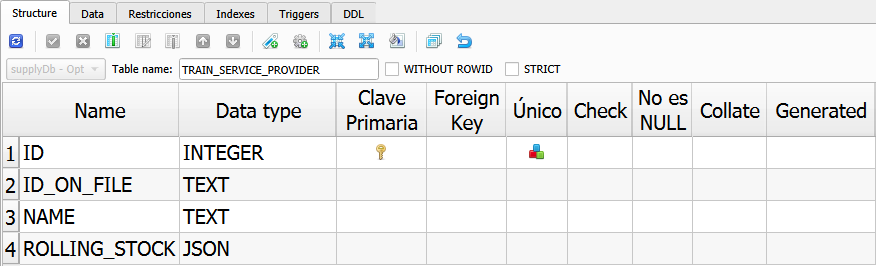
\includegraphics[width=.9\textwidth]{fig/Tablas base de datos/Oferta/TRAIN_SERVICE_PROVIDER.png}
\caption{Tabla \texttt{TRAIN\_SERVICE\_PROVIDER}}
\label{fig:dbSupplyTRAIN_SERVICE_PROVIDER}
\end{figure}
\newpage
Para almacenar las características de los trenes de los que disponen las diferentes compañías de servicios ferroviarios para la realización de los servicios ofertados, se emplea la tabla \texttt{ROLLING\_STOCK} (Figura~\ref{fig:dbSupplyROLLING_STOCK}), la cual cuenta con los campos: 
\begin{itemize}
    \item \texttt{ID}: Identificador autoincremental único de cada fila.
    \item \texttt{ID\_ON\_FILE}: Identificador que aparece en el archivo para cada material rodante.
    \item \texttt{NAME}: Nombre asignado al modelo de tren.
    \item \texttt{SEATS}: Diccionario en formato \acrshort{JSON} que almacena los diferentes tipos de asientos disponibles en el modelo de tren.
    \begin{itemize}
        \item La clave del diccionario representa el tipo de asiento.
        \item El valor asociado a cada clave indica la cantidad de asientos disponibles de ese tipo.
    \end{itemize}
\end{itemize}

\begin{figure}[H]
\centering
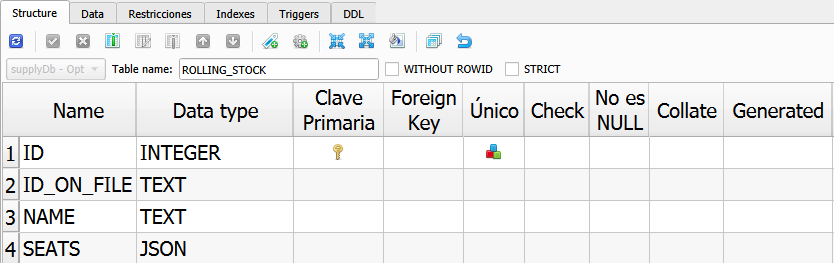
\includegraphics[width=.9\textwidth]{fig/Tablas base de datos/Oferta/ROLLING_STOCK.png}
\caption{Tabla \texttt{ROLLING\_STOCK}}
\label{fig:dbSupplyROLLING_STOCK}
\end{figure}

En la tabla \texttt{TIME\_SLOT} (Figura~\ref{fig:dbSupplyTIME_SLOT}) se almacenan los intervalos de tiempo de llegada y salida de los trenes de la estación. 

Esta tabla cuenta con tres campos: 
\begin{itemize}
    \item \texttt{ID}: Identificador único del intervalo.
    \item \texttt{START}: Hora de inicio del intervalo.
    \item \texttt{END}: Hora de finalización del intervalo.
\end{itemize}

\begin{figure}[H]
\centering
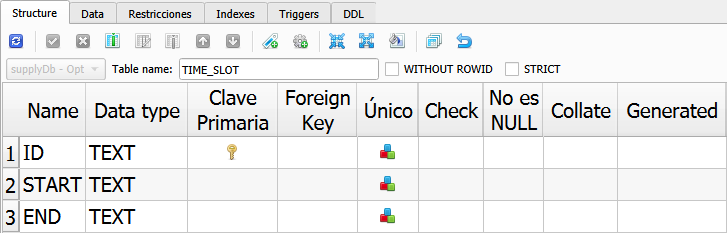
\includegraphics[width=.9\textwidth]{fig/Tablas base de datos/Oferta/TIME_SLOT.png}
\caption{Tabla \texttt{TIME\_SLOT}}
\label{fig:dbSupplyTIME_SLOT}
\end{figure}

La tabla \texttt{CORRIDOR} (Figura~\ref{fig:dbSupplyCORRIDOR}) almacena el identificador del corredor (\texttt{ID}) y el nombre que recibe el mismo (\texttt{NAME}), siendo los formatos de ambos campos texto plano.

\begin{figure}[H]
\centering
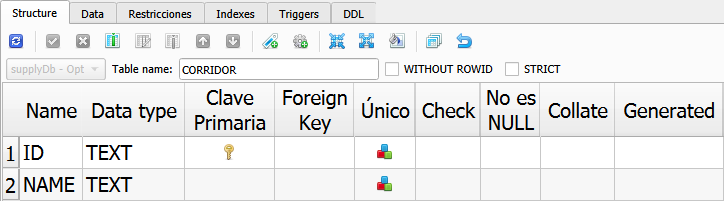
\includegraphics[width=.9\textwidth]{fig/Tablas base de datos/Oferta/CORRIDOR.png}
\caption{Tabla \texttt{CORRIDOR}}
\label{fig:dbSupplyCORRIDOR}
\end{figure}

Esta tabla está relacionada con \texttt{CORRIDOR\_STATIONS} (Figura~\ref{fig:dbSupplyCORRIDOR_STATIONS}), la cual almacena las estaciones presentes en el ramal del corredor (\texttt{STATIONS}), siendo el primer elemento de las listas la estación de inicio del ramal y el último elemento la estación donde finaliza el ramal del corredor. El campo \texttt{STATIONS} almacena los datos en formato \acrshort{JSON}.

\texttt{CORRIDOR\_STATIONS} se relaciona con las tablas \texttt{TESTS} y \texttt{CORRIDOR} mediante el empleo de claves foráneas en las columnas \texttt{TEST\_ID} y \texttt{CORRIDOR\_ID} respectivamente, cuyos datos se almacenan en formato de texto plano.

\begin{figure}[H]
\centering
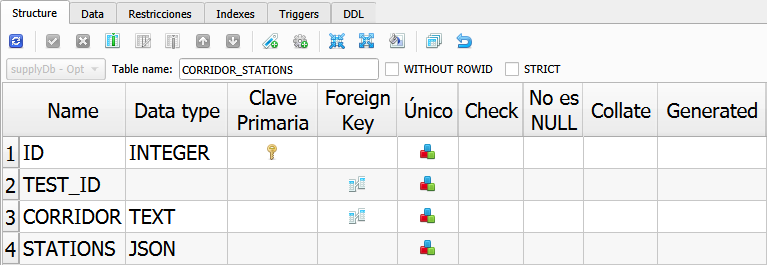
\includegraphics[width=.9\textwidth]{fig/Tablas base de datos/Oferta/CORRIDOR_STATIONS.png}
\caption{Tabla \texttt{CORRIDOR\_STATIONS}}
\label{fig:dbSupplyCORRIDOR_STATIONS}
\end{figure}

Los datos de los asientos que se ofertan por parte de las compañías de servicios ferroviarios se encuentran almacenados en la tabla \texttt{SEAT} (Figura~\ref{fig:dbSupplySEAT}). 

Esta tabla está compuesta de los siguientes campos: 
\begin{itemize}
    \item \texttt{ID}: Identificador autoincremental único de cada fila.
    \item \texttt{ID\_ON\_FILE}: Identificador que aparece en el archivo para cada tipo de asiento.
    \item \texttt{NAME}: Nombre asignado al asiento.
    \item \texttt{HARD\_TYPE}: Tipo de asiento según sus características físicas.
    \item \texttt{SOFT\_TYPE}: Tipo de servicios asociados al asiento.
\end{itemize}

\begin{figure}[H]
\centering
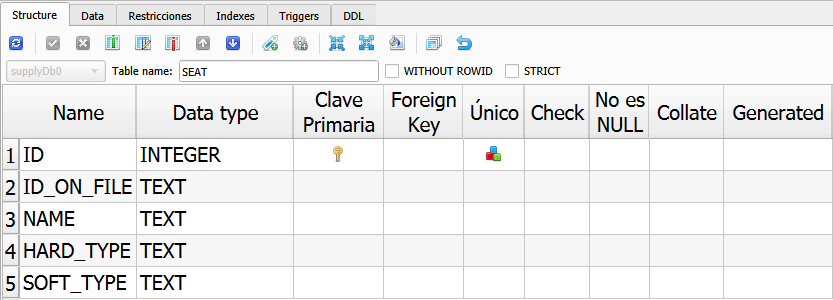
\includegraphics[width=.9\textwidth]{fig/Tablas base de datos/Oferta/SEAT.png}
\caption{Tabla \texttt{SEAT}}
\label{fig:dbSupplySEAT}
\end{figure}

La tabla \texttt{LINE} (Figura~\ref{fig:dbSupplyLINE}) contiene los datos de las diferentes líneas que componen los corredores por donde circulan los trenes. 

Esta tabla contiene las columnas:
\begin{itemize}
    \item \texttt{ID}: Identificador único de la línea.
    \item \texttt{NAME}: Nombre asignado a la línea.
    \item \texttt{CORRIDOR}: Clave foránea que referencia el identificador del corredor al que pertenece la línea.
\end{itemize}

Esta clave foránea relaciona la tabla \texttt{LINE} con la tabla \texttt{CORRIDOR} (Figura~\ref{fig:dbSupplyCORRIDOR}).

\begin{figure}[H]
\centering
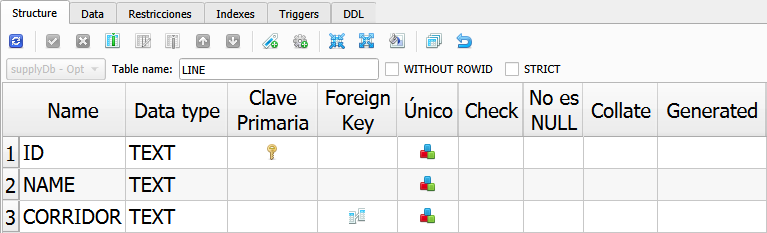
\includegraphics[width=.9\textwidth]{fig/Tablas base de datos/Oferta/LINE.png}
\caption{Tabla \texttt{LINE}}
\label{fig:dbSupplyLINE}
\end{figure}

En la tabla \texttt{STOPS} (Figura~\ref{fig:dbSupplySTOPS}) se almacenan las paradas que se realizan en las diferentes líneas ferroviarias. 

Esta tabla consta de los siguientes campos: 
\begin{itemize}
    \item \texttt{ID}: Identificador único de la parada.
    \item \texttt{TESTS\_ID}: Clave foránea que referencia el identificador almacenado en la tabla \texttt{TESTS} (Figura~\ref{fig:dbSupplyTESTS}).
    \item \texttt{LINE\_ID}: Clave foránea que referencia el identificador de la línea almacenado en la tabla \texttt{LINE} (Figura~\ref{fig:dbSupplyLINE}).
    \item \texttt{STATION}: Clave foránea que referencia el identificador de la estación almacenado en la tabla \texttt{STATIONS} (Figura~\ref{fig:dbSupplySTATIONS}).
    \item \texttt{ARRIVAL\_TIME}: Hora de llegada a la estación.
    \item \texttt{DEPARTURE\_TIME}: Hora de salida de la estación.
\end{itemize}

\begin{figure}[H]
\centering
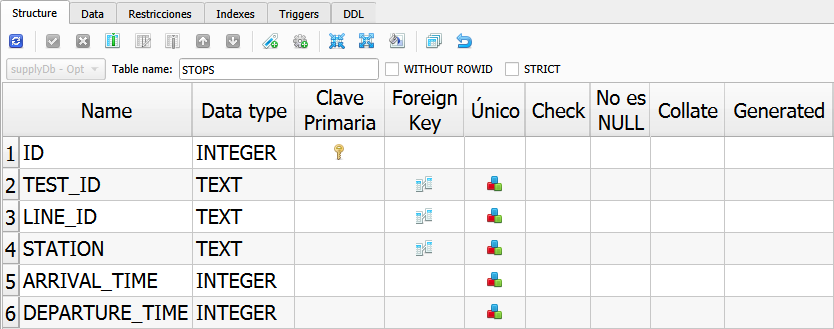
\includegraphics[width=.9\textwidth]{fig/Tablas base de datos/Oferta/STOPS.png}
\caption{Tabla \texttt{STOPS}}
\label{fig:dbSupplySTOPS}
\end{figure}

A continuación, se van a usar las tablas \texttt{LINE}~\ref{fig:dbSupplyLINE} y \texttt{STOPS} para realizar un ejemplo de cómo usar las relaciones que existen entre ambas para extraer datos en base a la intersección de ambas tablas usando el comando \acrshort{SQL} \texttt{INNER JOIN}. En este caso, la sentencia que aparece en el Listado~\ref{src:ejemploParadasLinea05065} seleccionará las paradas que se efectúan en la línea 05065 de entre todas las que existen en la tabla \texttt{STOPS}

\lstinputlisting[language=SQL, frame=none, numbers=none, basicstyle=\ttfamily\normalsize, caption={Sentencia para el ejemplo de uso de tablas auxiliares}, 
                 label=src:ejemploParadasLinea05065, inputencoding=utf8]{auxFiles/Querys de ejemplos/Paradas linea 05065.sql}

La tabla~\ref{tab:ejemploParadasLinea05065} contiene los datos seleccionados por la sentencia \acrshort{SQL} del Listado~\ref{src:ejemploParadasLinea05065}.

\begin{table}[H]
\centering
\begin{tabular}{c|c|c|c|c|c|}
\cline{2-6}
 & \cellcolor[HTML]{C0C0C0}ID
 & \cellcolor[HTML]{C0C0C0}LINE
 & \cellcolor[HTML]{C0C0C0}STATION
 & \cellcolor[HTML]{C0C0C0}ARRIVAL\_TIME
 & \cellcolor[HTML]{C0C0C0}DEPARTURE\_TIME \\ \hline
\multicolumn{1}{|l|}{1} & 1 & 05065 & 03216 & 0   & 0   \\ \hline
\multicolumn{1}{|l|}{2} & 2 & 05065 & 03213 & 25  & 27  \\ \hline
\multicolumn{1}{|l|}{3} & 3 & 05065 & 03208 & 61  & 63  \\ \hline
\multicolumn{1}{|l|}{4} & 4 & 05065 & 17000 & 126 & 126 \\ \hline
\end{tabular}
\caption{Paradas de la línea 05065}
\label{tab:ejemploParadasLinea05065}
\end{table}

Los datos de los diferentes servicios que se ofertan a lo largo del día se almacenan en la tabla \texttt{SERVICE} (Figura~\ref{fig:dbSupplySERVICE}). 

Estos datos se componen de: 
\begin{itemize}
    \item \texttt{ID}: Identificador único del servicio.
    \item \texttt{DATE}: Fecha en la que se realiza el servicio.
    \item \texttt{LINE}: Identificador de la línea en la que se lleva a cabo el servicio.
    \item \texttt{TIME\_SLOT}: Identificador del intervalo de tiempo asignado al servicio.
    \item \texttt{TRAIN\_SERVICE\_PROVIDER}: Identificador de la compañía que ofrece el servicio.
    \item \texttt{ROLLING\_STOCK}: Identificador de la máquina que realiza el servicio.
\end{itemize}

\begin{figure}[H]
\centering
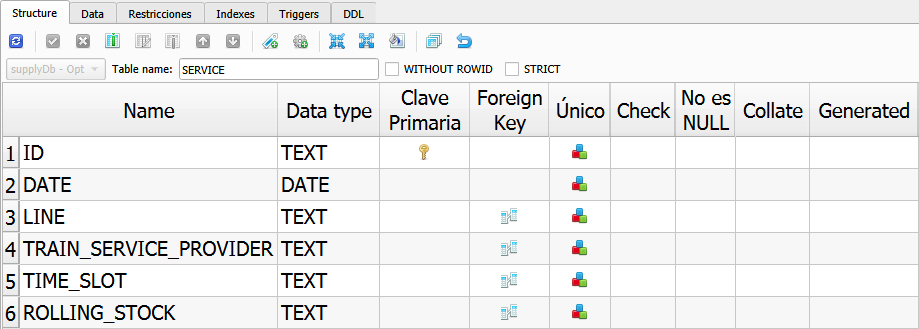
\includegraphics[width=.9\textwidth]{fig/Tablas base de datos/Oferta/SERVICE.png}
\caption{Tabla \texttt{SERVICE}}
\label{fig:dbSupplySERVICE}
\end{figure}

La tabla \texttt{RESTRICTIONS} (Figura~\ref{fig:dbSupplyRESTRICTIONS}) contiene las restricciones que tiene cada servicio, en este caso, restricciones de capacidad, ya que el simulador \acrshort{ROBIN} de momento solo acepta este tipo de restricciones. Tanto la tabla \texttt{RESTRICTIONS}, como el programa desarrollado, están preparados para aceptar otro tipo de restricciones.

Esta tabla cuenta con las columnas:
\begin{itemize}
    \item \texttt{ID}: Identificador auto-incremental de la restricción.
    \item \texttt{SERVICE\_ID}: Identificador del servicio al que esta asociada la restricción.
    \item \texttt{TYPE}: Tipo de restricción aplicada.
    \item \texttt{RESTRICTION:} Valor o conjunto de valores que definen la restricción.
\end{itemize}

Esta tabla está relacionada con la tabla \texttt{SERVICE} (Figura~\ref{fig:dbSupplySERVICE}), mediante el uso de la clave foránea \texttt{SERVICE\_ID}. 

\begin{figure}[H]
\centering
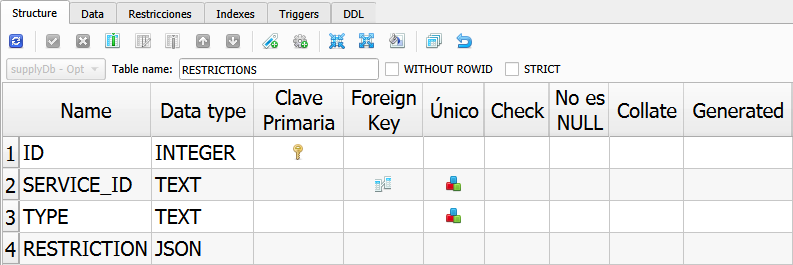
\includegraphics[width=.9\textwidth]{fig/Tablas base de datos/Oferta/RESTRICTIONS.png}
\caption{Tabla \texttt{RESTRICTIONS}}
\label{fig:dbSupplyRESTRICTIONS}
\end{figure}

En la tabla \texttt{ORIGIN\_DESTINATION\_TUPLES} se almacenan los datos de todos los trayectos ofrecidos en un servicio.  

Esta tabla contiene los siguientes campos:
\begin{itemize}
    \item \texttt{ID}: Identificador único de la tupla origen-destino.
    \item \texttt{TEST\_ID}: Clave foránea que referencia el identificador del archivo al que pertenece el servicio asociado a la tupla.
    \item \texttt{SERVICE\_ID}: Clave foránea que indica el identificador del servicio al que pertenece la tupla origen-destino.
    \item \texttt{ORIGIN}: Identificador de la estación de origen.
    \item \texttt{DESTINATION}: Identificador de la estación de destino.
    \item \texttt{SEATS}: Lista en formato \acrshort{JSON} que almacena los tipos de asientos para el trayecto entre origen y destino.
\end{itemize}

Las claves foráneas \texttt{TEST\_ID} y \texttt{SERVICE\_ID} establecen relaciones con las tablas \texttt{TESTS} (Figura~\ref{fig:dbSupplyTESTS}) y \texttt{SERVICE} (Figura~\ref{fig:dbSupplySERVICE}), respectivamente.

\begin{figure}[H]
\centering
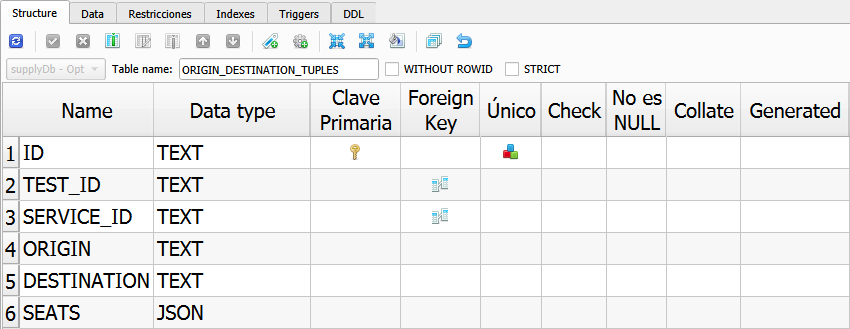
\includegraphics[width=.9\textwidth]{fig/Tablas base de datos/Oferta/ORIGIN_DESTINATION_TUPLES.png}
\caption{Tabla \texttt{ORIGIN\_DESTINATION\_TUPLES}}
\label{fig:dbSupplyODT}
\end{figure}

Los precios de los asientos ofertados en los diferentes servicios se almacenan en la tabla \texttt{SEATS\_PRICE} (Figura~\ref{fig:dbSupplySEATS_PRICE}). Esta tabla contiene los siguientes campos:
\begin{itemize}
    \item \texttt{ID}: Identificador único de cada asiento.
    \item \texttt{ODT\_ID}: Clave foránea que referencia el identificador de la tupla origen-destino a la que pertenece el asiento.
    \item \texttt{SEAT}: Identificador del tipo de asiento.
    \item \texttt{PRICE}: Precio asignado al asiento para un trayecto determinado por \texttt{ODT\_ID}.
\end{itemize}

La tabla \texttt{SEATS\_PRICE} se relaciona con \texttt{ORIGIN\_DESTINATION\_TUPLES} mediante la clave foránea \texttt{ODT\_ID}.

\begin{figure}[H]
\centering
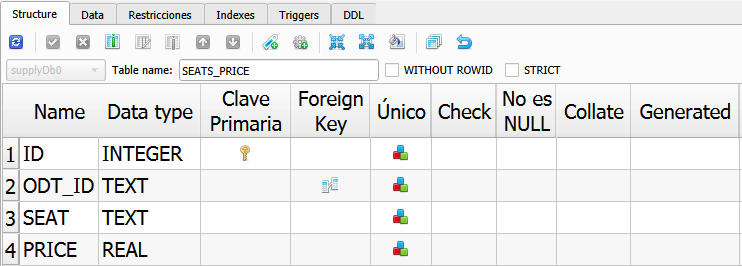
\includegraphics[width=.9\textwidth]{fig/Tablas base de datos/Oferta/SEATS_PRICE.png}
\caption{Tabla \texttt{SEATS\_PRICE}}
\label{fig:dbSupplySEATS_PRICE}
\end{figure}

\subsubsection{Tablas auxiliares}

Las tablas auxiliares tienen como cometido relacionar los diferentes archivos con los datos almacenados en las demás tablas de la base de datos y así evitar que haya datos duplicados. Esto permite que en cada archivo se pueda determinar qué datos de las diferentes tablas corresponden a ese archivo.  

En la tabla \texttt{AUX\_STATIONS} (Figura~\ref{fig:dbSupplyAUX_STATIONS}) se establecen las relaciones entre los archivos y las estaciones incluidas en el conjunto de datos de cada archivo. 

\begin{figure}[H]
\centering
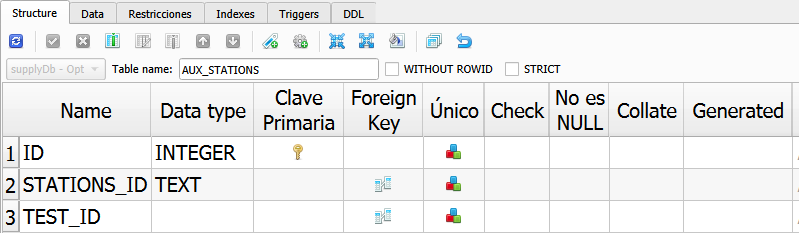
\includegraphics[width=.9\textwidth]{fig/Tablas base de datos/Oferta/AUX_STATIONS.png}
\caption{Tabla \texttt{AUX\_STATIONS}}
\label{fig:dbSupplyAUX_STATIONS}
\end{figure}

En \texttt{AUX\_TRAIN\_SERVICE\_PROVIDER} (Figura~\ref{fig:dbSupplyAUX_TRAIN_SERVICE_PROVIDER}) se establecen las relaciones entre los archivos y los proveedores de servicio ferroviario. Gracias a ello, se puede definir a qué archivo pertenecen los diferentes proveedores de servicios ferroviarios.

\begin{figure}[H]
\centering
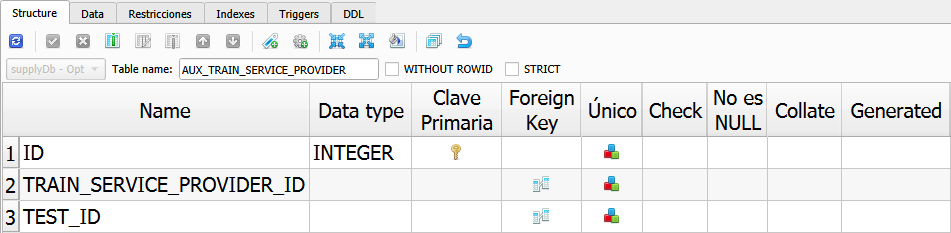
\includegraphics[width=.9\textwidth]{fig/Tablas base de datos/Oferta/AUX_TRAIN_SERVICE_PROVIDER.png}
\caption{Tabla \texttt{AUX\_TRAIN\_SERVICE\_PROVIDER}}
\label{fig:dbSupplyAUX_TRAIN_SERVICE_PROVIDER}
\end{figure}

\texttt{AUX\_ROLLING\_STOCK} (Figura~\ref{fig:dbSupplyAUX_ROLLING_STOCK}) vincula los archivos con el material rodante (rolling stock), relacionando así el archivo con el material rodante que aparece en dicho archivo.

\begin{figure}[H]
\centering
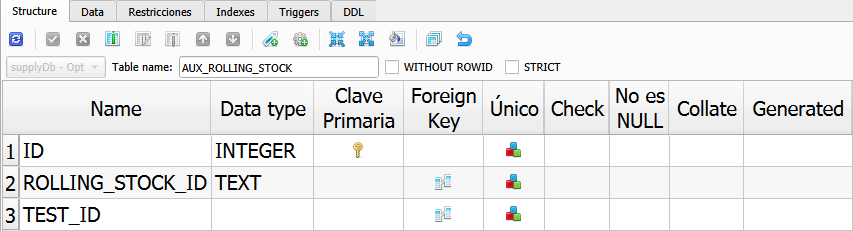
\includegraphics[width=.9\textwidth]{fig/Tablas base de datos/Oferta/AUX_ROLLING_STOCK.png}
\caption{Tabla \texttt{AUX\_ROLLING\_STOCK}}
\label{fig:dbSupplyAUX_ROLLING_STOCK}
\end{figure}

La tabla \texttt{AUX\_TIME\_SLOT} (Figura~\ref{fig:dbSupplyAUX_TIME_SLOT}) asocia cada archivo con los intervalos de tiempo (time slots) pertenecientes a cada uno de los archivos. 

\begin{figure}[H]
\centering
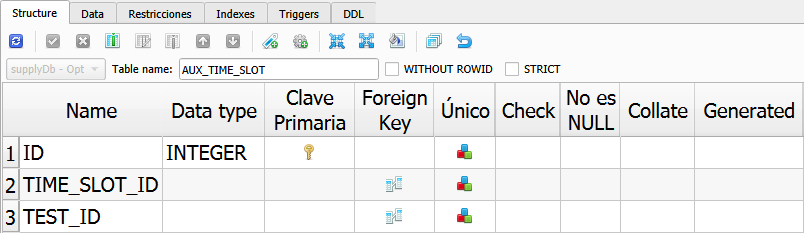
\includegraphics[width=.9\textwidth]{fig/Tablas base de datos/Oferta/AUX_TIME_SLOT.png}
\caption{Tabla \texttt{AUX\_TIME\_SLOT}}
\label{fig:dbSupplyAUX_TIME_SLOT}
\end{figure}

En la tabla \texttt{AUX\_CORRIDOR} (Figura~\ref{fig:dbSupplyAUX_CORRIDOR}) se asocia cada archivo con corredores específicos relacionados con cada uno de los archivos.

\begin{figure}[H]
\centering
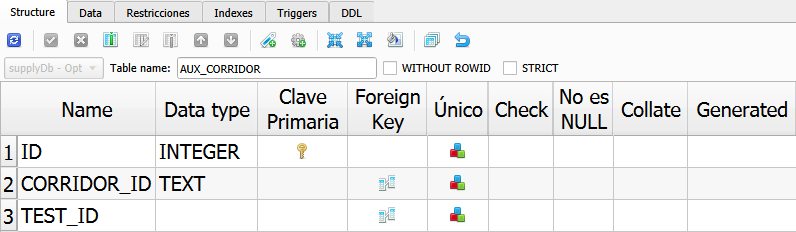
\includegraphics[width=.9\textwidth]{fig/Tablas base de datos/Oferta/AUX_CORRIDOR.png}
\caption{Tabla \texttt{AUX\_CORRIDOR}}
\label{fig:dbSupplyAUX_CORRIDOR}
\end{figure}

\texttt{AUX\_SEAT} (Figura~\ref{fig:dbSupplyAUX_SEAT}) indica qué tipos de asientos se emplean en los diferentes archivos que pueda albergar la base de datos.

\begin{figure}[H]
\centering
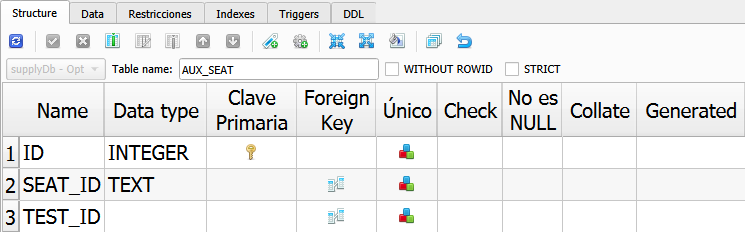
\includegraphics[width=.9\textwidth]{fig/Tablas base de datos/Oferta/AUX_SEAT.png}
\caption{Tabla \texttt{AUX\_SEAT}}
\label{fig:dbSupplyAUX_SEAT}
\end{figure}

Por último, la tabla \texttt{AUX\_SERVICE} (Figura~\ref{fig:dbSupplyAUX_SERVICE}) relaciona los diferentes servicios almacenados en la tabla \texttt{SERVICE} (Figura~\ref{fig:dbSupplySERVICE}) con los archivos que emplean los datos de dichos servicios.

\begin{figure}[H]
\centering
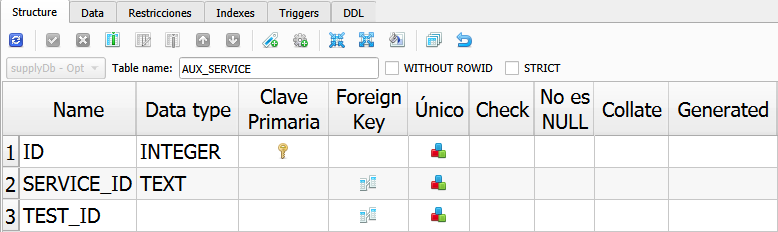
\includegraphics[width=.9\textwidth]{fig/Tablas base de datos/Oferta/AUX_SERVICE.png}
\caption{Tabla \texttt{AUX\_SERVICE}}
\label{fig:dbSupplyAUX_SERVICE}
\end{figure}

A continuación se va a exponer un ejemplo de uso de las tablas auxiliares para extraer los datos de los servicios del archivo \acrshort{Yaml} con el nombre \href{https://github.com/Sergioba99/TFG-Gestor_De_Bases_de_Datos/blob/master/Archivos%20Yaml%20y%20CSV/Originales/Oferta/supply_03216_60000_2025-06-02_2025-06-16.yaml}{"supply\_03216\_60000\_2025-06-02\_2025-06-16"}\footnote{\textbf{Archivo "supply\_03216\_60000\_2025-06-02\_2025-06-16.yaml":} \url{https://github.com/Sergioba99/TFG-Gestor_De_Bases_de_Datos/blob/master/Archivos\%20Yaml\%20y\%20CSV/Originales/Oferta/supply_03216_60000_2025-06-02_2025-06-16.yaml}}. Este archivo se encuentra subido al repositorio de GitHub. Empleando la sentencia \acrshort{SQL} del Listado~\ref{src:ejemploUsoTablasAuxiliares} se han obtenido todos los servicios pertenecientes al archivo mencionado.

\lstinputlisting[language=SQL, frame=none, numbers=none, basicstyle=\ttfamily\normalsize, caption={Sentencia para el ejemplo de uso de tablas auxiliares}, 
                 label=src:ejemploUsoTablasAuxiliares, inputencoding=utf8]{auxFiles/Querys de ejemplos/Ejemplo de uso de tablas auxiliares.sql}

Dado que la lista de servicios seleccionados mediante la sentencia \acrshort{SQL} del Listado~\ref{src:ejemploUsoTablasAuxiliares} es extensa, se ha cogido una muestra de 5 filas, la cual aparece en la Tabla~\ref{tab:ejemploTablasAuxiliares}. El archivo que contiene todas las entradas generadas mediante la sentencia \acrshort{SQL} del Listado~\ref{src:ejemploUsoTablasAuxiliares} se encuentra en el siguiente \href{https://github.com/Sergioba99/TFG-Gestor_De_Bases_de_Datos/blob/master/Archivos%20Yaml%20y%20CSV/Exportados/Vistas%20exportadas/Ejemplo%20de%20uso%20de%20tablas%20auxiliares%20largo.csv}{enlace}\footnote{\textbf{Archivo CSV completo:} \url{https://github.com/Sergioba99/TFG-Gestor_De_Bases_de_Datos/blob/master/Archivos\%20Yaml\%20y\%20CSV/Exportados/Vistas\%20exportadas/Ejemplo\%20de\%20uso\%20de\%20tablas\%20auxiliares\%20largo.csv}} del repositorio de GitHub.

\begin{table}[H]
\centering
\resizebox{\textwidth}{!}{
\begin{tabular}{c|c|c|c|c|c|c|}
\cline{2-7}
 & \cellcolor[HTML]{C0C0C0}ID
 & \cellcolor[HTML]{C0C0C0}DATE
 & \cellcolor[HTML]{C0C0C0}LINE
 & \cellcolor[HTML]{C0C0C0}TRAIN\_SERVICE\_PROVIDER
 & \cellcolor[HTML]{C0C0C0}TIME\_SLOT
 & \cellcolor[HTML]{C0C0C0}ROLLING\_STOCK \\ 
\hline
\multicolumn{1}{|l|}{1} & 05065\_02-06-2025-06.32 & 2025-06-02 & 05065 & 1 & 39210 & 1 \\ \hline
\multicolumn{1}{|l|}{2} & 05065\_03-06-2025-06.32 & 2025-06-03 & 05065 & 1 & 39210 & 1 \\ \hline
\multicolumn{1}{|l|}{3} & 05065\_04-06-2025-06.32 & 2025-06-04 & 05065 & 1 & 39210 & 1 \\ \hline
\multicolumn{1}{|l|}{4} & 05065\_05-06-2025-06.32 & 2025-06-05 & 05065 & 1 & 39210 & 1 \\ \hline
\multicolumn{1}{|l|}{5} & 05065\_06-06-2025-06.32 & 2025-06-06 & 05065 & 1 & 39210 & 1 \\ \hline
\end{tabular}}
\caption{Muestra de datos obtenidos de la sentencia del Listado~\ref{src:ejemploUsoTablasAuxiliares}}
\label{tab:ejemploTablasAuxiliares}
\end{table}

\subsection{Base de datos para los archivos de entrada de datos de la demanda}
\label{subsec:dBDemand}
La base de datos que almacena la información de la demanda consta de 12 tablas. La organización de estas se puede encontrar en el \acrshort{EDR} (Figura~\ref{fig:edrDemandaSimplificado}). Una versión más extendida de dicho \acrshort{EDR}, que contiene también los nombres de las columnas de cada una de las tablas, puede encontrarse en el Anexo~\ref{fig:edrDemanda}. En esta base de datos se guardan los datos relacionados con la modelización de los patrones de demanda de los diferentes tipos de usuarios previstos para emplearlos en el simulador \acrshort{ROBIN}.

\begin{figure}[H]
\centering
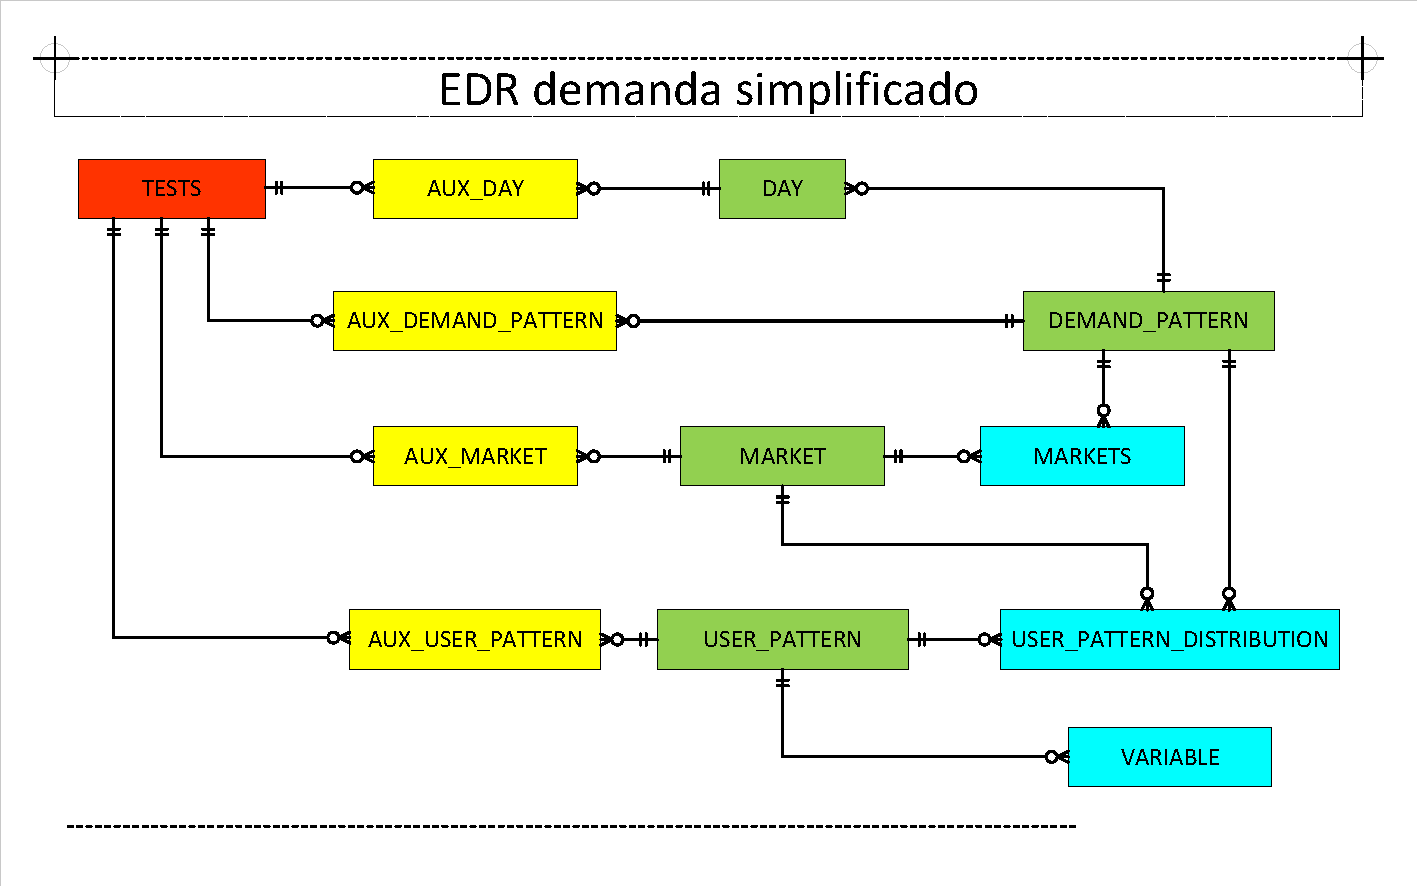
\includegraphics[width=.95\textwidth]{fig/Bases de datos/EDR demanda simplificado.pdf}
\caption{Esquema de la base de datos de la demanda. En naranja aparece la tabla principal, en amarillo las tablas auxiliares, en verde las tablas de datos y en azul las tablas de datos auxiliares.}
\label{fig:edrDemandaSimplificado}
\end{figure}

La tabla principal de la base de datos aparece representada con el color naranja y tiene la finalidad de almacenar el nombre de los archivos \acrshort{Yaml} de entrada de datos de la demanda y las observaciones que el usuario considere relevantes.

Las tablas auxiliares aparecen en color amarillo y relacionan los datos pertenecientes al archivo de entrada de datos de la demanda, almacenados en la base de datos, con el archivo en sí. Esto se realiza mediante el uso del identificador que posee la fila de la tabla principal en la que se almacena el nombre del archivo y los identificadores de las filas con los datos pertenecientes a ese archivo. Como ya se ha comentado en la base de datos de los archivos de entrada de datos de la oferta, esto se ha diseñado así para evitar elementos repetidos en las tablas de datos, optimizando así el espacio ocupado por los datos dentro de la base de datos.

Las tablas de datos, en color verde, están destinadas a almacenar los datos referenciados por las diferentes claves raíz dentro del archivo \acrshort{Yaml} de entrada de datos de la demanda, por ejemplo los patrones de usuario o los patrones de demanda. Al igual que sucede en la base de datos de los datos de la oferta, si alguna clave dentro del archivo \acrshort{Yaml} tiene asociada una estructura compleja (como una lista de listas o una lista de diccionarios, entre otras) los datos que se encuentren dentro de estas estructuras se almacenan en las tablas auxiliares de datos, en color azul claro. Estructuras más simples como una lista o un diccionario, si que se almacenan dentro de las tablas de datos como texto en formato \acrshort{JSON}, como por ejemplo, la lista de reglas difusas que definen el comportamiento del patrón de usuario bajo la clave \texttt{rules} definida en la clave raíz \texttt{userPattern} o los diferentes conjuntos que componen las variables lingüísticas.

A continuación se muestra cada una de las tablas que componen la base de datos.

\subsubsection{Tabla principal}

Al igual que ocurría con la base de datos para los archivos de configuración de la oferta, la tabla principal será la de \texttt{TESTS}, la cual albergará los campos:
\begin{itemize}
    \item \texttt{ID}: Identificador único que se le asigna a cada archivo.
    \item \texttt{NAME}: Nombre del archivo de configuración introducido a la base de datos.
    \item \texttt{OBSERVATIONS}: Observaciones proporcionadas por el usuario.
\end{itemize}

\begin{figure}[H]
\centering
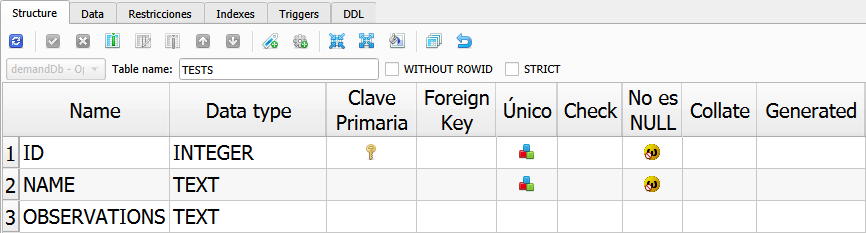
\includegraphics[width=.9\textwidth]{fig/Tablas base de datos/Demanda/TESTS.png}
\caption{Tabla \texttt{TESTS}}
\label{fig:dbDemandTESTS}
\end{figure}

\subsubsection{Tablas de datos}

La tabla \texttt{DEMAND\_PATTERN} (Figura~\ref{fig:dbDemandDEMAND_PATTERN}) contiene el identificador del patrón de demanda (\texttt{ID}), así como el nombre que recibe el patrón de demanda (\texttt{NAME}). 

\begin{figure}[H]
\centering
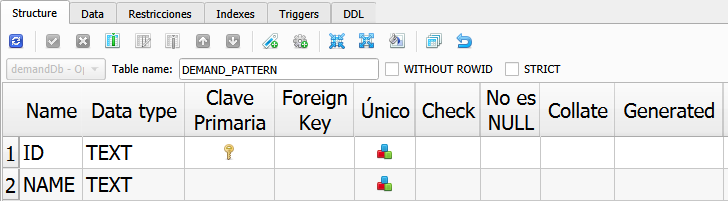
\includegraphics[width=.9\textwidth]{fig/Tablas base de datos/Demanda/DEMAND_PATTERN.png}
\caption{Tabla \texttt{DEMAND\_PATTERN}}
\label{fig:dbDemandDEMAND_PATTERN}
\end{figure}

\texttt{MARKET} (Figura~\ref{fig:dbDemandMARKET}) contiene los datos que definen los diferentes mercados posibles, es decir, los  diferentes trayectos posibles entre las estaciones que se van a estudiar. La tabla \texttt{MARKET} cuenta con los siguientes campos:

\begin{itemize}
    \item \texttt{ID}: Identificador único que recibe cada mercado.
    \item \texttt{DEPARTURE\_STATION}: Nombre de la estación de salida.
    \item \texttt{DEPARTURE\_STATION\_COORDS}: Coordenadas de la estación de salida almacenadas como una lista en formato \acrshort{JSON}.
    \item \texttt{ARRIVAL\_STATION}: Nombre de la estación de destino.
    \item \texttt{ARRIVAL\_STATION\_COORDS}: Coordenadas de la estación de destino almacenadas como una lista en formato \acrshort{JSON}.
\end{itemize}

\begin{figure}[H]
\centering
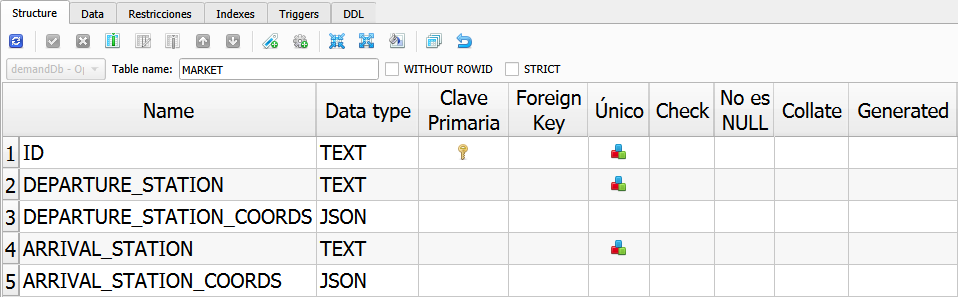
\includegraphics[width=.9\textwidth]{fig/Tablas base de datos/Demanda/MARKET.png}
\caption{Tabla \texttt{MARKET}}
\label{fig:dbDemandMARKET}
\end{figure}

En \texttt{MARKETS} (Figura~\ref{fig:dbDemandMARKETS}) se almacenan los diferentes mercados que pertenecen a los patrones de demanda de \texttt{DEMAND\_PATTERN}. Esta tabla contiene las siguientes columnas:

\begin{itemize}
    \item \texttt{DEMAND\_PATTERN\_ID}: Clave foránea perteneciente al identificador de un patrón de demanda.
    \item \texttt{MARKET}: Clave foránea que hace referencia a un mercado en específico.
    \item \texttt{POTENTIAL\_DEMAND}: Función empleada en el simulador para el cálculo de la posible demanda.
    \item \texttt{POTENTIAL\_DEMAND\_KWARGS}: Argumentos para la función del calculo de la posible demanda.
\end{itemize}
Esta tabla se relaciona con las tablas \texttt{DEMAND\_PATTERN} (Figura~\ref{fig:dbDemandDEMAND_PATTERN}) y \texttt{MARKET} (Figura~\ref{fig:dbDemandMARKET}), mediante el uso de las claves foráneas \texttt{DEMAND\_PATTERN\_ID} y \texttt{MARKET} respectivamente.

\begin{figure}[htbp]
\centering
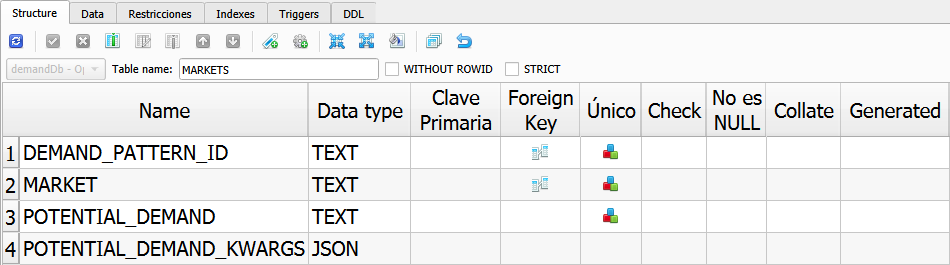
\includegraphics[width=.9\textwidth]{fig/Tablas base de datos/Demanda/MARKETS.png}
\caption{Tabla \texttt{MARKETS}}
\label{fig:dbDemandMARKETS}
\end{figure}

Los datos de los patrones que pueden seguir los usuarios se almacenan en la tabla \texttt{USER\_PATTERN} (Figura~\ref{fig:dbDemandUSER_PATTERN}). Esta tabla consta de las siguientes columnas:
\begin{itemize}
    \item \texttt{ID}: Identificador que recibe el patrón de usuario.
    \item \texttt{NAME}: Nombre del patrón de usuario.
    \item \texttt{RULES}: Diccionario en formato \acrshort{JSON} que almacena las reglas difusas que después se emplearan en la simulación.
    \item \texttt{ARRIVAL\_TIME}: Función para generar una distribución de los diferentes tiempos de llegada que prefiere un patrón de usuario determinado.
    \item \texttt{ARRIVAL\_TIME\_KWARGS}: Parámetros para la función definida en \texttt{ARRIVAL\_TIME}.
    \item \texttt{PURCHASE\_DAY}: Función que genera el número de días de antelación con los que un tipo de usuario realizará la compra de sus billetes.
    \item \texttt{PURCHASE\_DAY\_KWARGS}: Parámetros para la función definida en \texttt{PURCHASE\_DAY}.
    \item \texttt{FORBIDDEN\_DEPARTURE\_HOURS}: Franja horaria durante la cual el usuario prefiere no iniciar su viaje.
    \item \texttt{SEATS}: Diccionario en \acrshort{JSON} que contiene los datos de utilidad de cada tipo de asiento para un tipo de usuario.
    \item \texttt{TRAIN\_SERVICE\_PROVIDERS}: Diccionario que almacena los datos de utilidad de los diferentes proveedores de servicios ferroviarios para cada tipo de usuario. Probabilidad de que el usuario adquiera un billete que le resulta útil sin realizar una búsqueda exhaustiva.
    \item \texttt{UTILITY\_THRESHOLD}: Umbral de utilidad para el patrón de usuario.
    \item \texttt{ERROR}: Función para generar una distribución del error cometido.
    \item \texttt{ERROR\_KWARGS}: Parámetros para la función definida en \texttt{ERROR}.
\end{itemize}

\begin{figure}[H]
\centering
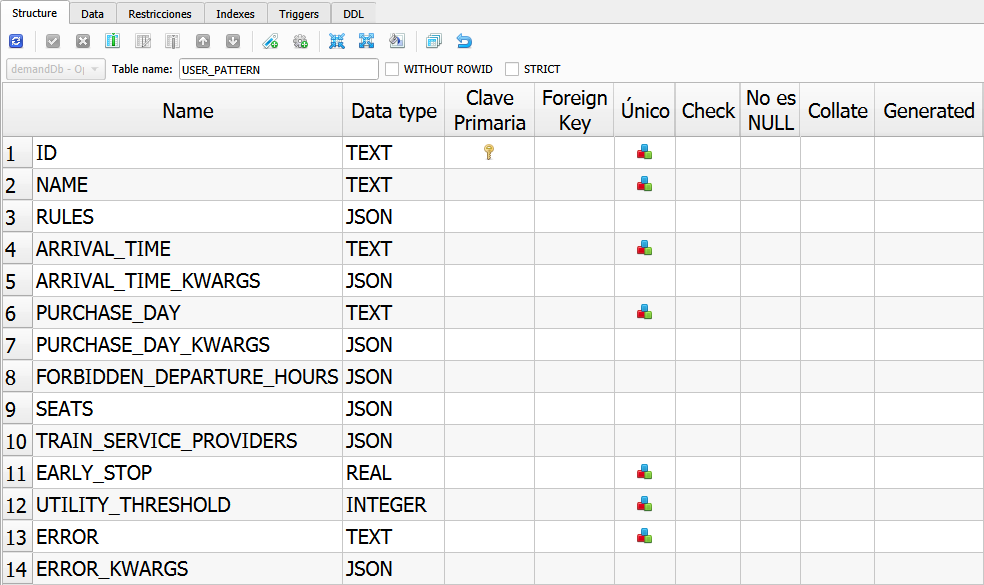
\includegraphics[width=.9\textwidth]{fig/Tablas base de datos/Demanda/USER_PATTERN.png}
\caption{Tabla \texttt{USER\_PATTERN}}
\label{fig:dbDemandUSER_PATTERN}
\end{figure}

La tabla \texttt{VARIABLE} (Figura~\ref{fig:dbDemandVARIABLE}) contiene las diferentes variables difusas que se emplean en la simulación para cada tipo de patrón de usuario. Las columnas que esta tabla posee son las siguientes:
\begin{itemize}
    \item \texttt{USER\_PATTERN\_ID}: Clave foránea que referencia al identificador del patrón de usuario (\texttt{USER\_PATTERN}).
    \item \texttt{NAME}: Nombre que recibe la variable difusa.
    \item \texttt{TYPE}: Tipo de variable difusa, que puede ser de dos categorías: \texttt{fuzzy} o \texttt{categorical}.
    \item \texttt{SUPPORT}: Lista con dos valores en formato \acrshort{JSON} que define el intervalo de la variable difusa. Este campo solo se completa cuando la variable es de tipo \texttt{fuzzy}.
    \item \texttt{SETS}: Diccionario que almacena los diferentes conjuntos difusos. La clave del diccionario es el nombre del conjunto, mientras que el valor asociado es una lista que representa el dominio del conjunto difuso.
    \item \texttt{LABELS}: Lista de etiquetas asociadas a las variables de tipo \texttt{categorical}. Este campo contendrá datos únicamente cuando el tipo de la variable sea \texttt{categorical}.
\end{itemize}

La tabla \texttt{VARIABLE} tiene una única relación con la tabla \texttt{USER\_PATTERN} (Figura~\ref{fig:dbDemandUSER_PATTERN}) mediante la clave foránea \texttt{USER\_PATTERN\_ID}.

\begin{figure}[H]
\centering
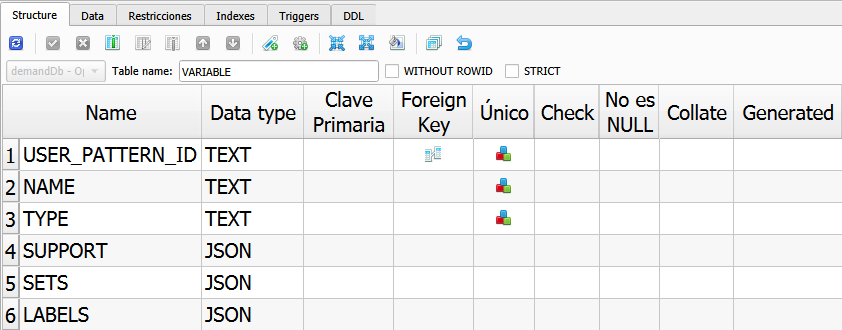
\includegraphics[width=.9\textwidth]{fig/Tablas base de datos/Demanda/VARIABLE.png}
\caption{Tabla \texttt{VARIABLE}}
\label{fig:dbDemandVARIABLE}
\end{figure}

En \texttt{DAY} se relaciona un patrón de demanda con el día que se ofrecen los servicios ferroviarios. Esta tabla cuenta con:
\begin{itemize}
    \item \texttt{ID}: Identificador único para el día.
    \item \texttt{DATE}: Fecha en la que se aplica el patrón de demanda.
    \item \texttt{DEMMAND\_PATTERN}: Clave foránea que relaciona el día con un patrón de demanda mediante el \texttt{ID} de la tabla \texttt{DEMAND\_PATTERN}.
\end{itemize}
\texttt{DAY} tiene una relación con la tabla \texttt{DEMAND\_PATTERN} (Figura~\ref{fig:dbDemandDEMAND_PATTERN}) mediante el empleo de la clave foránea \texttt{DEMMAND\_PATTERN}.

\begin{figure}[H]
\centering
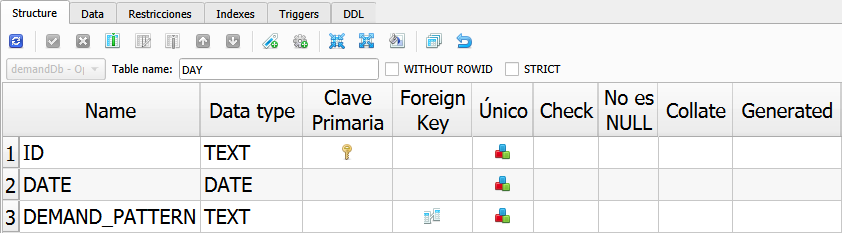
\includegraphics[width=.9\textwidth]{fig/Tablas base de datos/Demanda/DAY.png}
\caption{Tabla \texttt{DAY}}
\label{fig:dbDemandDAY}
\end{figure}

\texttt{USER\_PATTERN\_DISTRIBUTION} almacena los datos de la distribución de los diferentes patrones de usuario para determinados patrones de demanda. \texttt{USER\_PATTERN\_DISTRIBUTION} consta de las siguientes columnas:
\begin{itemize}
    \item \texttt{MARKET\_ID}: Clave foránea que relaciona el \texttt{ID} de un mercado con \texttt{USER\_PATTERN\_DISTRIBUTION}.
    \item \texttt{DEMAND\_PATTERN\_ID}: Clave foránea que relaciona un patrón de demanda usando el identificador de este.
    \item \texttt{USER\_PATTERN\_ID}: Clave foránea que relaciona un patrón de usuario mediante el \texttt{ID} de \texttt{USER\_PATTERN}. 
    \item \texttt{PERCENTAGE}: Porcentaje de un tipo de usuario que se espera para un determinado patrón de demanda.
\end{itemize}
La tabla \texttt{USER\_PATTERN\_DISTRIBUTION} se relaciona con las tablas \texttt{MARKET} (Figura~\ref{fig:dbDemandMARKET}), \texttt{DEMAND\_PATTERN} (Figura~\ref{fig:dbDemandDEMAND_PATTERN}) y \texttt{USER\_PATTERN} (Figura~\ref{fig:dbDemandUSER_PATTERN}) mediante las claves foráneas \texttt{MARKET\_ID}, \texttt{DEMAND\_PATTERN\_ID} y \texttt{USER\_PATTERN\_ID}.

\begin{figure}[H]
\centering
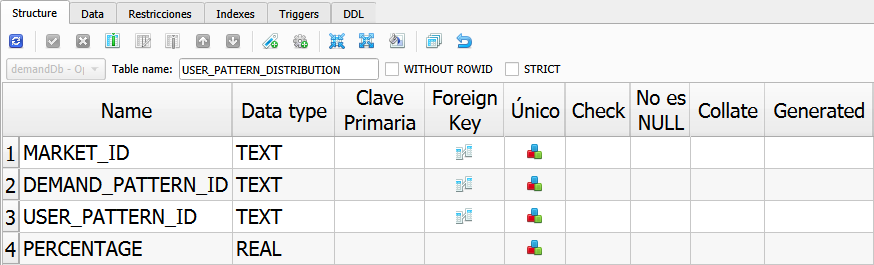
\includegraphics[width=.9\textwidth]{fig/Tablas base de datos/Demanda/USER_PATTERN_DISTRIBUTION.png}
\caption{Tabla \texttt{USER\_PATTERN\_DISTRIBUTION}}
\label{fig:dbDemandUSER_PATTERN_DISTRIBUTION}
\end{figure}

\subsubsection{Tablas auxiliares}

Las tablas auxiliares están diseñadas para vincular cada archivo con los datos almacenados en las demás tablas de la base de datos, evitando la duplicación de información. Gracias a esta estructura, es posible determinar con precisión qué registros corresponden a cada archivo sin necesidad de replicar los datos en múltiples instancias.

La tabla \texttt{AUX\_DEMAND\_PATTERN} (Figura~\ref{fig:dbDemandAUX_DEMAND_PATTERN}) vincula los archivos con los distintos patrones de demanda que puedan estar almacenados en la tabla \texttt{DEMAND\_PATTERN} (Figura~\ref{fig:dbDemandDEMAND_PATTERN}). 

\begin{figure}[H]
\centering
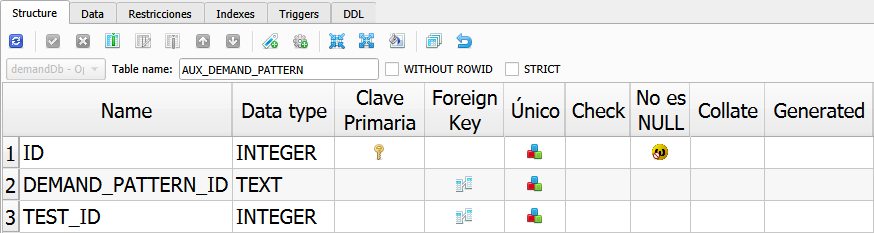
\includegraphics[width=.9\textwidth]{fig/Tablas base de datos/Demanda/AUX_DEMAND_PATTERN.png}
\caption{Tabla \texttt{AUX\_DEMAND\_PATTERN}}
\label{fig:dbDemandAUX_DEMAND_PATTERN}
\end{figure}

\texttt{AUX\_MARKET} (Figura~\ref{fig:dbDemandAUX_MARKET}) establece la relación entre los archivos y los mercados que forman parte de la tabla \texttt{MARKET} (Figura~\ref{fig:dbDemandMARKET}).

\begin{figure}[H]
\centering
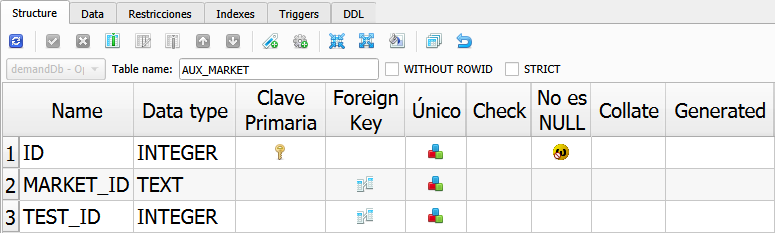
\includegraphics[width=.9\textwidth]{fig/Tablas base de datos/Demanda/AUX_MARKET.png}
\caption{Tabla \texttt{AUX\_MARKET}}
\label{fig:dbDemandAUX_MARKET}
\end{figure}

En \texttt{AUX\_USER\_PATTERN} (Figura~\ref{fig:dbDemandAUX_USER_PATTERN}) se gestionan las relaciones entre los archivos y los distintos patrones de usuario contenidos en \texttt{USER\_PATTERN} (Figura~\ref{fig:dbDemandUSER_PATTERN}). 

\begin{figure}[H]
\centering
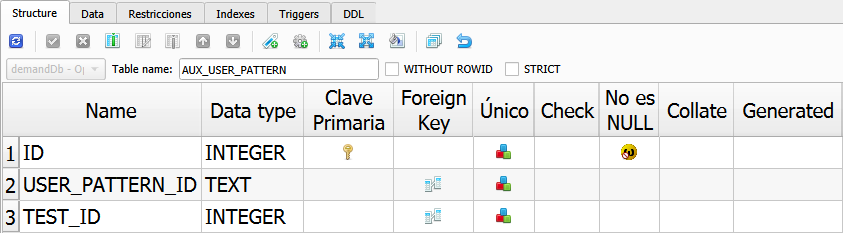
\includegraphics[width=.9\textwidth]{fig/Tablas base de datos/Demanda/AUX_USER_PATTERN.png}
\caption{Tabla \texttt{AUX\_USER\_PATTERN}}
\label{fig:dbDemandAUX_USER_PATTERN}
\end{figure}

\texttt{AUX\_DAY} (Figura~\ref{fig:dbDemandAUX_DAY}) relaciona los archivos con los días específicos en los que se ejecutan las pruebas que están almacenados en la tabla \texttt{DAY} (Figura~\ref{fig:dbDemandDAY}). 

\begin{figure}[H]
\centering
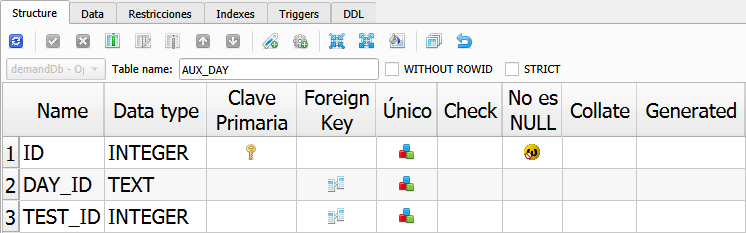
\includegraphics[width=.9\textwidth]{fig/Tablas base de datos/Demanda/AUX_DAY.png}
\caption{Tabla \texttt{AUX\_DAY}}
\label{fig:dbDemandAUX_DAY}
\end{figure}

\subsection{Base de datos para la configuración de los resultados}
\label{subsec:dBResults}
 La base de datos destinada a almacenar los resultados consta de tres tablas, organizadas conforme al \acrshort{EDR} (Figura~\ref{fig:edrResultadosSimplificado}). Una versión más extendida de dicho \acrshort{EDR}, que contiene también los nombres de las columnas de cada una de las tablas, puede encontrarse en el Anexo~\ref{fig:edrResultados}. Su propósito es registrar los datos generados por el simulador \acrshort{ROBIN}.


\begin{figure}[H]
\centering
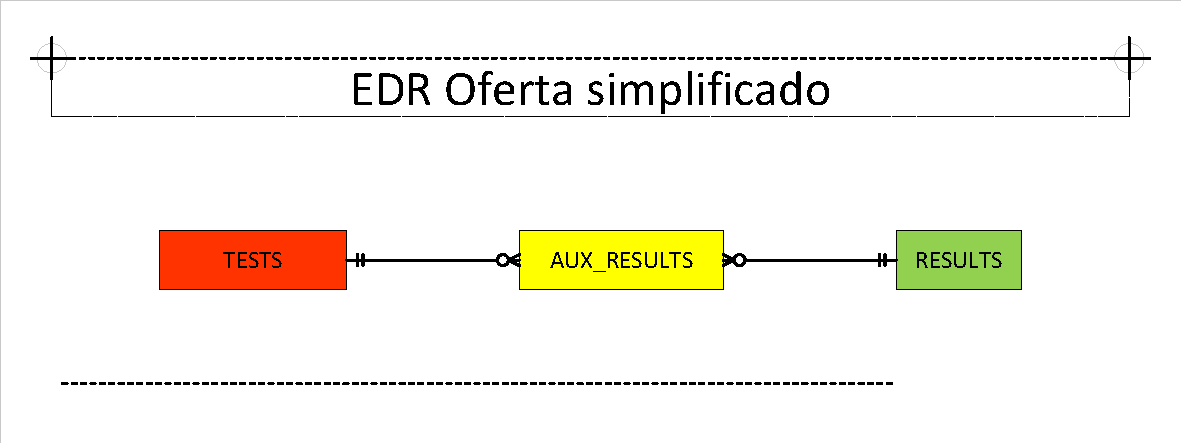
\includegraphics[width=.9\textwidth]{fig/Bases de datos/EDR resultados simplificado.pdf}
\caption{Esquema de la base de datos de los resultados. En naranja aparece la tabla principal, en amarillo la tabla auxiliar y en verde la tabla de datos.}
\label{fig:edrResultadosSimplificado}
\end{figure}

La tabla principal de la base de datos, en naranja, tiene como objetivo almacenar el nombre del archivo \acrshort{CSV} de resultados importado a la base de datos y las observaciones que un usuario realice sobre el mismo.

La tabla auxiliar, en color amarillo, relaciona los datos almacenados en la tabla de datos con los archivos que posean dichos datos. Esto se realiza mediante los identificadores de las filas que contienen los datos y el identificador asignado a cada uno de los archivos durante la importación de la información.

La tabla de datos almacena los datos provenientes del archivo \acrshort{CSV} importado. Debido a que los archivos \acrshort{CSV} son tablas, no poseen ninguna estructura compleja, por lo que en esta base de datos no hay ninguna tabla auxiliar de datos.

A continuación se muestra cada una de las tablas que componen esta base de datos.

\subsubsection{Tabla principal}

Al igual que ocurre con la base de datos para los archivos de entrada de la oferta y de la demanda, la tabla principal será la de \texttt{TESTS} y tiene los siguientes campos:
\begin{itemize}
    \item \texttt{ID}: Identificador único que se le asigna a cada archivo.
    \item \texttt{NAME}: Nombre del archivo de configuración introducido a la base de datos.
    \item \texttt{OBSERVATIONS}: Observaciones proporcionadas por el usuario.
\end{itemize}

\begin{figure}[H]
\centering
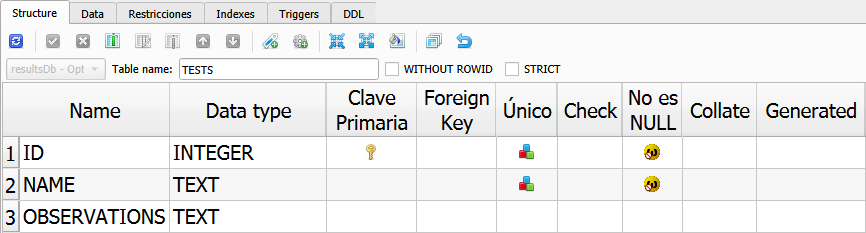
\includegraphics[width=.9\textwidth]{fig/Tablas base de datos/Resultados/TESTS.png}
\caption{Tabla \texttt{TESTS}}
\label{fig:dbResultsTESTS}
\end{figure}

\subsubsection{Tablas de datos}

La tabla \texttt{RESULTS} (Figura~\ref{fig:dbResultsRESULTS}) contendrá los datos de los resultados de las simulaciones, realizadas con el simulador \acrshort{ROBIN} y consta de las siguientes columnas:
\begin{itemize}
    \item \texttt{ID}: Identificador de cada uno de los resultados.
    \item \texttt{USER\_PATTERN}: Patrón de usuario empleado.
    \item \texttt{DEPARTURE\_STATION}: Estación de salida de la simulación.
    \item \texttt{ARRIVAL\_STATION}: Estación de llegada empleado en la simulación.
    \item \texttt{ARRIVAL\_DAY}: Día de llegada en la simulación.
    \item \texttt{ARRIVAL\_TIME}: Tiempo relativo en el que el tren llega a la estación.
    \item \texttt{PURCHASE\_DAY}: Días de antelación de la compra de los billetes.
    \item \texttt{SERVICE}: Identificador del servicio que se ha simulado.
    \item \texttt{SERVICE\_DEPARTURE\_TIME}: Hora prevista de salida del servicio.
    \item \texttt{SERVICE\_ARRIVAL\_TIME}: Hora prevista de llegada del servicio.
    \item \texttt{SEAT}: Tipo de asiento comprado por el usuario.
    \item \texttt{PRICE}: Precio pagado por el usuario.
    \item \texttt{UTILITY}: Porcentage que describe como de útil es el resultado para el tipo de usuario.
    \item \texttt{BEST\_SERVICE}: Servicio que mejor se adapta a los patrones de usuario y demanda.
    \item \texttt{BEST\_SEAT}: Asiento que mejor se adapta a los patrones de usuario y demanda.
    \item \texttt{BEST\_UTILITY}: Valor más alto de utilidad alcanzado durante la simulación.
\end{itemize}

\begin{figure}[H]
\centering
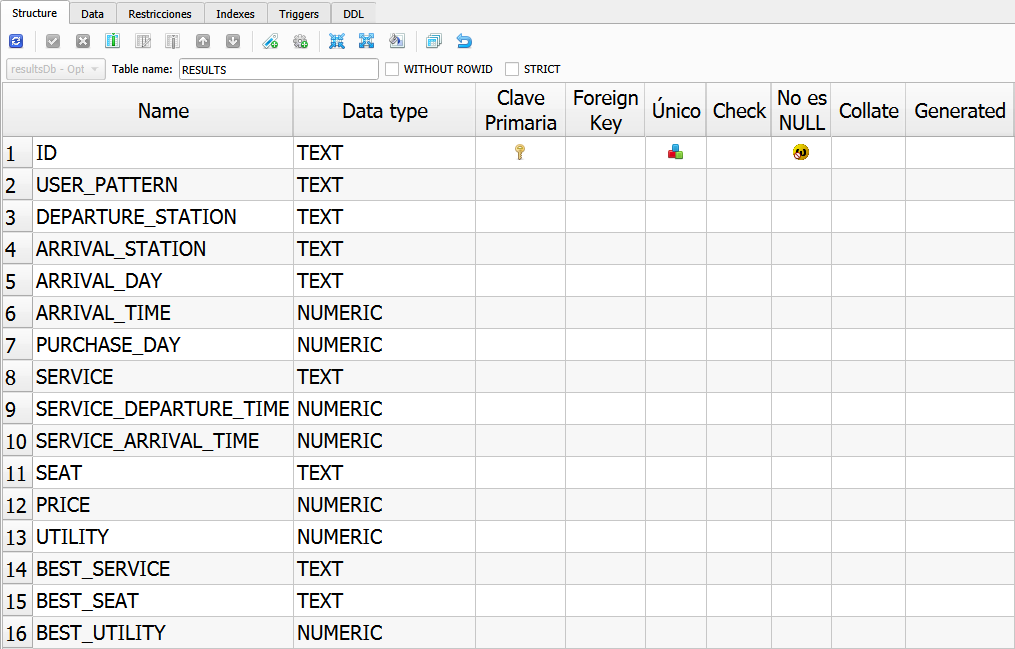
\includegraphics[width=.9\textwidth]{fig/Tablas base de datos/Resultados/RESULTS.png}
\caption{Tabla \texttt{RESULTS}}
\label{fig:dbResultsRESULTS}
\end{figure}

\subsubsection{Tablas auxiliares}

La tabla \texttt{AUX\_RESULTS} (Figura~\ref{fig:dbResultsAUX_RESULTS}) vincula los archivos con los distintos resultados de los tests simulados que se encuentran en la tabla \texttt{RESULTS} (Figura~\ref{fig:dbResultsRESULTS}). 

\begin{figure}[H]
\centering
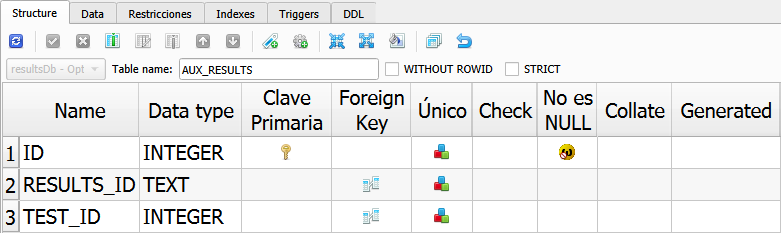
\includegraphics[width=.9\textwidth]{fig/Tablas base de datos/Resultados/AUX_RESULTS.png}
\caption{Tabla \texttt{AUX\_RESULTS}}
\label{fig:dbResultsAUX_RESULTS}
\end{figure}